\documentclass[psamsfonts]{amsart}
\usepackage[utf8]{inputenc}
\usepackage{amsfonts, comment, enumerate}
\usepackage[mathcal]{eucal}
\usepackage[hidelinks]{hyperref}
\hypersetup{
pdftitle={Complexity of deep computations via topology of function spaces}
pdfsubject={Mathematics, Set Theory},
pdfauthor={Luciano Salvetti, Tonatiuh Matos-Wiederhold},
pdfkeywords={}
}
\usepackage{amsmath}
\usepackage{xcolor}
\usepackage{amsthm}
\usepackage{pdflscape}
\usepackage{pgfplots}
\usepackage{mathrsfs}
%\usepackage{euler}
\usepackage{tikz}
\usetikzlibrary{trees}

\newtheorem{thm}{Theorem}[section]
\newtheorem{cor}[thm]{Corollary}
\newtheorem{prop}[thm]{Proposition}
\newtheorem{lem}[thm]{Lemma}
\newtheorem{conj}[thm]{Conjecture}
\newtheorem{quest}[thm]{Question}
\newtheorem*{claim}{Claim}
\newtheorem{fact}[thm]{Fact}
\newtheorem{ppty}[thm]{Property}


\theoremstyle{definition}
\newtheorem{defn}[thm]{Definition}
\newtheorem{question}[thm]{Question}
\newtheorem{defns}[thm]{Definitions}
\newtheorem{con}[thm]{Construction}
\newtheorem{exmp}[thm]{Example}
\newtheorem{exmps}[thm]{Examples}
\newtheorem{notn}[thm]{Notation}
\newtheorem{notns}[thm]{Notations}
\newtheorem{addm}[thm]{Addendum}
\newtheorem{exer}[thm]{Exercise}
\newtheorem{limit}[thm]{Limitation}

\theoremstyle{remark}
\newtheorem{rem}[thm]{Remark}
\newtheorem{rems}[thm]{Remarks}
\newtheorem{warn}[thm]{Warning}
\newtheorem{sch}[thm]{Scholium}

\makeatletter
\let\c@equation\c@thm
\makeatother
\numberwithin{equation}{section}

%\bibliographystyle{plain}

%--------Meta Data: Fill in your info------
\title[Complexity of deep computations via topology of function spaces]{Complexity of deep computations\\ via topology of function spaces}

\author[Dueñez, Iovino, Matos-Wiederhold, Salvetti, Tall]{
Eduardo Dueñez$^{1}$ \qquad
José Iovino$^{1}$ \qquad
Tonatiuh Matos-Wiederhold$^{2}$ \qquad
Luciano Salvetti$^{2}$ \qquad
Franklin D. Tall$^{2}$
}

\usepackage{lineno}
\linenumbers

\begin{document}

\maketitle

{\centering\tiny\vspace{-0.6cm}
$^{1}$Department of Mathematics, University of Texas at San Antonio\\
$^{2}$Department of Mathematics, University of Toronto\\
}

\begin{abstract}
We study complexity of deep computations. We use topology of function spaces, specifically, the classification Rosenthal compacta, to identify new complexity classes.  We use the language of model theory, specifically,  the concept of  the independence from Shelah's classification theory,  to translate between topology and computation.
%This paper revisits and extends a bridge between functional analysis and model theory, emphasizing its relevance to the theoretical foundations of machine learning. We show that the compactness behavior of families of Baire class 1 Bourgain-Fremlyn-Talagrand dichotomyfunctions mirrors the learnability conditions in the sense of \emph{Probably Approximately Correct} (PAC) learning, and that the failure of compactness corresponds to the presence of infinite \emph{Vapnik-Chervonenkis} (VC) dimension. From this perspective, Rosenthal compacta emerge as the natural topological counterpart of PAC-learnable concept classes, while NIP vs. IP structures capture the precise boundary between analytical regularity and combinatorial intractability. These parallels suggest a unified framework linking compactness, definability, and learnability, exemplifying how the topology of function spaces encodes the algorithmic and epistemic limits of prediction.
\end{abstract}

\maketitle

\setcounter{section}{-1}


\section{Introduction}


In this paper we study limit behavior of real-valued computations as the value of certain parameters  of the computation model tend towards infinity, or towards zero, or towards some other fixed value, e.g.,  the depth of a neural network tending to infinity, or the time interval between layers of the network tending toward zero. Recently, particular cases of this situation have attracted considerable attention in deep learning research (e.g., Neural Ordinary Differential Equations~\cite{Chen:2018}, Physics-Informed Neural Networks~\cite{Raissi-Perdikaris-Karniadakis:2019},  deep equilibrium models~\cite{Bai:2019}, among others). In this paper, we combine ideas of topology, measure theory, and  model theory to study these limit phenomena from a unified viewpoint. 

Informed by model theory, to each computation in a given computation model, we associate a continuous real-valued function, called the \emph{type} of the computation, that describes the logical properties of this computation with respect to the rest of the model. This allows us to view computations in any given computational model  as elements of a space of real-valued functions, which is called the \emph{space of types} of the model. The idea of embedding models of theories into their type spaces is central in model theory. The embedding of computations into spaces of types allows us to utilize the vast theory of topology of function spaces, known as $C_p$-theory, to obtain results about complexity of topological limits of computations. As we shall indicate next, recent classification results for spaces of functions provide an elegant and powerful machinery to classify computations according to their levels of ``tameness’’ or ``wildness’’, with the former corresponding roughly to polynomial approximability and the latter to exponential approximability. The viewpoint of spaces of types, which we have borrowed from model theory, thus becomes a ``Rosetta stone’’  that allows us  to interconnect various classification programs: In topology, the classification of Rosenthal compacta pioneered by Todorčević~\cite{Todorcevic_1999_CompactSubsetsBaire}; in logic, the classification of theories developed by Shelah~\cite{Shelah:1990}; and in statistical learning, the notion PAC learning and VC dimension pioneered by Vapkins and Chervonenkis~\cite{Vapnik-Chervonenkis:1974, Vapnik-Chervonenkis:1971}. 


In a previous paper~\cite{alva2024approximability}, we introduced the concept of limits of computations, which we called \emph{ultracomputations} (given they arise as ultrafilter limits of standard computations) and \emph{deep computations}  (following usage in machine learning~\cite{Bai:2019}). There is a technical difference between both designations, but in this paper, to simplify the nomenclature, we will ignore the difference and use only the term ``deep computation’’.

In \cite{alva2024approximability}, we proved a new ``tame vs wild'' (i.e., polynomial vs exponential) dichotomy for complexity of deep computations by invoking a classical result of Grothendieck from late 50s~\cite{Grothendieck:1952}. Under our model-theoretic Rosetta stone, polynomial approximability in the sense of computation becomes identified with the notion of continuous extendability in the sense of topology, and with the notions of \emph{stability} and \emph{type definability} in the sense of model theory.

 In this paper, we follow a more general approach, i.e., we view deep computations as pointwise limits of continuous functions. In topology functions that arise as the pointwise limit of a sequence of continuous are called \emph{functions of the first Baire class}, or \emph{Baire class~1} functions, or \emph{Baire-1} for short; Baire class~1 form a step above simple continuity in the hierarchy of functions studied in real analysis  (Baire class 0 functions being continuous functions). Intuitively, Baire-1 functions represent functions with ``controlled'' discontinuities, so they are  crucial in topology and set theory.

We prove a new ``tame vs wild'' Ramsey-theoretic dichotomy for complexity of general deep computations by invoking a famous paper by Bourgain, Fremlin and Talagrand from the late 70s~\cite{BFT_1978_PCompactBaire}, and  a new trichotomy for the class of ``tame'' deep computations by invoking an equally celebrated result of Todorčević, from the late 90s, for  functions of the first Baire class~\cite{Todorcevic_1999_CompactSubsetsBaire}.

Todorčević’s trichotomy regards \emph{Rosenthal compacta}; these  are special classes of  topological spaces, defined as compact spaces that can be embedded (homeomorphically identified as a subset) within the space of Baire class 1 functions on some Polish (separable, complete metric) space, under the pointwise convergence topology. Rosenthal compacta  exhibit  ``topological tameness," meaning that they behave in relatively controlled ways, and since the late 70's, they have played a crucial role for understanding complexity of structures of functional analysis, especially, Banach spaces. Todorčević’s trichotomy has been utilized to settle longstanding problems in topological dynamics and topological entropy~\cite{glasner2022tame}.

Through our Rosetta stone, Rosenthal compacta in topology correspond to the important concept of  ``No Independence Property" (known as ``NIP’’) in model theory, identified by Shelah~\cite{Shelah:1971,Shelah:1990}, and to the concept of  Probably Approximately Correct learning (known as ``PAC learnability'') in statistical learning theory identified by Valiant~\cite{Valiant:1984}. 

Going beyond Todorčević’s trichotomy, we invoke a more recent heptachotomy for Rosenthal compacta obtained by Argyros, Dodos and Kanellopoulos~\cite{argyros2008rosenthal}. Argyros, Dodos and Kanellopoulos identified seven fundamental ``prototypes" of separable Rosenthal compacta, and  proved that any non-metrizable separable Rosenthal compactum must contain a ``canonical" embedding of one of these prototypes. They showed that if a separable Rosenthal compactum is not hereditarily separable, it must contain an uncountable discrete subspace of the size of the continuum.


We believe that the results presented in this paper show practitioners of computation, or topology, or descriptive set theory, or  model theory, how classification invariants used in their field translate into classification invariants of other fields. However, in the interest of accessibility, we do not assume previous familiarity with high-level topology or model theory, or computing. The only technical prerequisite of the paper is undergraduate-level topology and measure theory. The necessary topological background beyond undergraduate topology is covered in section~\ref{sec:prelim}.

In section \ref{sec:prelim}, we present the basic topological and combinatorial preliminaries, and in section and \ref{S:CCS}, we introduce the structural/model-theoretic viewpoint (no previous exposure to model theory is needed). Section~\ref{S:Classification} is devoted to the classification of deep computations. The final section, section~\ref{Measure-theoretic NIP} presents the probabilistic viewpoint.


Throughout the paper, we focus on classical computation; however, by refining the model-theoretic tools, the results presented here can be extended to quantum computation and open quantum systems. This extension will be addressed in a forthcoming paper.

\tableofcontents

\begin{comment}

\section{Technical and historical backround}

Suppose that $A$ is a subset of the real line $\mathbb R$ and that $\overline A$ is its \emph{closure}. It is a well-known fact that any point of closure of $A$, say $x\in\overline A$, can be \emph{approximated} by points inside of $A$, in the sense that a sequence $\{x_n\}_{n\in\mathbb N}\subseteq A$ must exist with the property that $\lim_{n\to\infty}x_n=x$. For most applications we wish to approximate objects more complicated than points, such as functions.

Suppose we wish to build a neural network that decides, given an 8 by 8 black-and-white image of a hand-written scribble, what single decimal digit the scribble represents. Maybe there exists $f$, a function representing an optimal solution to this classifier. Thus if $X$ is the set of all (possible) images, then for $I\in X$, $f(I)\in\{0,1,2,\dots,9\}$ is the ``best'' (or ``good enough'' for whatever deployment is needed) possible guess. Training the neural network involves approximating $f$ until its guesses are within an acceptable error range. In general, $f$ might be a function defined on a more complicated topological space $X$.

Often computers' viable operations are restricted (addition, subtraction, multiplication, division, etc.) and so we want to approximate a complicated function using simple functions (like polynomials). The problem is that, in contrast with mere points, functions in the closure of a set of functions need not be approximable (meaning the pointwise limit of a sequence of functions) by functions in the set.

Functions that are the pointwise limit of continuous functions are \emph{Baire class 1 functions}, and the set of all of these is denoted by $B_1(X)$. Notice that these are not necessarily continuous themselves! A set of Baire class 1 functions, $A$, will be relatively compact if its closure consists of just Baire class 1 functions (we delay the formal definition of \emph{relatively compact} until Section~\ref{sec:prelim}, but the fact mentioned here is sufficient). The Bourgain-Fremlin-Talagrand (BFT) theorem reveals a precise correspondence between relative compactness in $B_1(X)$ and the model-theoretic notion of \emph{Non-Independence Property} (NIP). This was realized by Pierre Simon in \cite{Simon_2015_RosenthalNIP}. 

Simon's insight was to view definable families of functions as sets of real-valued functions on type spaces and to interpret relative compactness in $B_1(X)$ as a form of ``tame behavior'' under ultrafilter limits. From this perspective, NIP theories are those whose definable families behave like relatively compact sets of Baire class 1 functions, avoiding the wild, $\beta\mathbb N$-like configurations that witness instability. This observation opened a new bridge between analysis and logic: topological compactness corresponds to the absence of combinatorial independence. Simon's later developments connected these ideas to \emph{Keisler measures} and \emph{empirical averages}, allowing tools from functional analysis to be used to study learnability and definable types. This reinterpretation of model-theoretic tameness through the lens of the BFT theorem has made NIP a central notion not only in stability theory but also in contemporary connections with learning theory and ergodic analysis.

Historically, the notion of NIP arises from Shelah's foundational work on the classification theory of models. In his seminal book \emph{Unstable Theories}~\cite{shelah1978unstable}, Shelah introduced the independence property as a key dividing line within unstable structures, identifying the class of \emph{stable} theories inside those in which this property fails. Fix a first-order formula $\varphi(x,y)$ in a language $L$ and a model $M$ of an $L$-theory $T$. We say that $\varphi(x,y)$ has the \emph{independence property (IP)} in $M$ if there is a sequence $(c_i)_{i\in\mathbb N}\subseteq M^{|x|}$ such that for every $S\subseteq\mathbb N$ there is $a_S\in M^{|y|}$ with $$\forall i\in\mathbb N,\qquad M\models\varphi(c_i,a_S)\quad\iff\quad i\in S.$$ The formula $\phi(x,y)$ has the IP if it does so in some model $M$, and the formula has the \emph{non-independence property (NIP)} if it does not have the IP. The latter notion of NIP generalizes stability by forbidding the full combinatorial independence pattern while allowing certain controlled forms of unstability. Thus, Simon's interpretation of the BFT theorem can be viewed as placing Shelah's dividing line into a topological-analytic framework, connecting the earliest notions of stability to compactness phenomena in spaces of Baire class 1 functions.

One of the most important innovations in Machine Learning is the mathematical notion, introduced by Turing Awardee Leslie Valiant in the 1980s, of ‘probably approximately correct learning’, or PAC-learning for short~\cite{bendavid2019understanding}. We give a standard but short overview of these concepts in the context that is relevant to this work.

Consider the following important idea in data classification. Suppose that $A$ is a set and that $\mathcal C$ is a collection of sets. We say that $\mathcal C$ \emph{shatters} $A$ if every subset of $A$ is of the form $C\cap A$ for some $C\in\mathcal C$. For a classical geometric example, if $A$ is the set of four points on the Euclidean plane of the form $(\pm1,\pm1)$, then the collection of all half-planes does not shatter $A$, the collection of all open balls does not shatter $A$, but the collection of all convex sets shatters $A$. While $A$ need not be finite, it will usually be assumed to be so in Machine Learning applications. A finer way to distinguish collections of sets that shatter a given set from those that do not is by the \emph{Vapnik-Chervonenkis dimension (VC-dimension)}, which is equal to the cardinality of the largest finite set shattered by the collection, in case it exists, or to infinity otherwise.

A concrete illustration of these ideas appears when considering threshold classifiers on the real line. Let $\mathcal{H}$ be the collection of all indicator functions $h_t$ given by $h_t(x)=1$ if $x\leq t$ and $h_t(x)=0$ otherwise. Each $h_t$ is a Baire class 1 function, and the family $\mathcal{H}$ is relatively compact in $B_1(\mathbb{R})$. In model-theoretic terms, $\mathcal{H}$ is NIP, since no configuration of points and thresholds can realize the full independence pattern of a binary matrix. By contrast, the family of parity functions $\{x\mapsto (-1)^{\langle w,x\rangle}:w\in\{0,1\}^n\}$ on $\{0,1\}^n$ (here ${\langle w,x\rangle}$ is the usual vector dot product) has the independence property and fails relative compactness in $B_1(X)$, capturing the analytical meaning of instability. This dichotomy mirrors the behavior of concept classes with finite versus infinite VC dimension in statistical learning theory.

Going back to the model theoretic framework, let $$\mathcal F_\varphi(M):=\{\varphi(M,a):a\in M^{|y|}\}$$ be the family of subsets of $M^{|x|}$ defined by instances of the formula $\varphi$, where $\varphi(M,a)$ is the set of $|x|$-tuples $c$ in $M$ for which $M\models \varphi(c,a)$. The fundamental theorem of statistical learning states that a binary hypothesis class is PAC-learnable if and only if it has finite VC-dimension, and the subsequent theorem connects the rest of the concepts presented in this section.

\begin{thm}[Laskowski]
    The formula $\varphi(x,y)$ satisfies the NIP if and only if $\mathcal F_\varphi(M)$ has finite VC-dimension.
\end{thm}

For two simple examples of formulas satisfying the NIP, consider first the language $L=\{<\}$ and the model $M=(\mathbb R,<)$ of the reals with their usual linear order. Take the formula $\varphi(x,y)$ to mean $x<y$, then $\varphi(M,a)=(-\infty,a)$, and so $\mathcal F_\varphi(M)$ is just the set of left open rays. The VC-dimension of this collection is 1, since it can shatter a single point, but no two point set can be shattered since the rays are downwards closed. Now in contrast, the collection of open intervals, given by the formula $\varphi(x;y_1,y_2):=(y_1<x)\land(x<y_2)$, has VC-dimension 2.

In this work, we study the corresponding notions of NIP (and hence PAC-learnability) in the context of Compositional Computation Structures (CCS) introduced in \cite{alva2024approximability}.

\end{comment}

\section{General topological preliminaries: From continuity to Baire class 1}
\label{sec:prelim}

In this section we give preliminaries from general topology and function space theory. We include some of the proofs for completeness, but the reader familiar with these topics may skip them.

Recall that a subset of a topological space is $F_\sigma$ if it is a countable union of closed  sets, and $G_\delta$ if it is a countable intersection of closed sets. Note that in a metrizable space, every open set is $F_\sigma$; equivalently, every closed set is $G_\delta$.

A \emph{Polish space} is a separable and completely metrizable topological space. The most important examples are the reals $\mathbb R$, the Cantor space $2^\mathbb N$ (the set of all infinite binary sequences, endowed with the product topology), and the Baire space $\mathbb N^\mathbb N$ (the set of all infinite sequences of naturals, also with the product topology). Countable products of Polish spaces are Polish; this includes spaces like $\mathbb R^\mathbb N$, the space of sequences of real numbers. 

In this paper, we shall discuss  subspaces, and so there is a pertinent subtlety of the definitions worth mentioning: \emph{completely metrizable space} is not the same as \emph{complete metric space}; for an illustrative example, the interval $(0,1)$ with  the metric inherited from the reals not complete, but it is Polish since that is homeomorphic to the real line. Being Polish is a topological property.

The following result is a cornerstone of descriptive set theory, closely tied to the work of Wacław Sierpiński and Kazimierz Kuratowski, with proofs often built upon their foundations and formalized later, notably, involving Stefan Mazurkiewicz's work on complete metric spaces.

\begin{fact}
A subset \(A\) of a Polish space \(X\) is itself Polish in the subspace topology if and only if it is a  $G_{\delta }$ set. In particular, closed subsets and open subsets of Polish spaces are also Polish spaces.
\end{fact}

Given two topological spaces $X$ and $Y$ we denote by $C_p(X,Y)$ the set of all continuous functions $f:X\rightarrow Y$ endowed with the topology of pointwise convergence. When $Y=\mathbb{R}$, we denote this collection simply as $C_p(X)$.
 A natural question is, how do topological properties of $X$ translate into $C_p(X)$ and vice versa? These questions, and in general the study of these spaces, are the concern of $C_p$-theory, an active field of research in general topology which was pioneered by A. V. Arhangel’skiĭ and his students in the 1970's and 1980's. This field has found many applications in model theory and functional analysis. Recent surveys on the topics include \cite{hamel2023cp} and \cite{tkachuk2011cp}.
 
 A  \emph{Baire class 1} function between topological spaces is a function that can be expressed as the pointwise limit of a sequence of continuous functions. If $X$ nd $Y$ are topological spaces,  the Baire class 1 functions $f:X\rightarrow Y$ endowed with the topology of pointwise convergence is denoted $B_1(X,Y)$. As above, in the special case $Y=\mathbb{R}$ we denote $B_1(X,Y)$. as  $B_1(X)$. Clearly, $C_p(X,Y)\subseteq B_1(X,Y)$.  The Baire hierarchy of functions was introduced by René-Louis Baire in his 1899 doctoral thesis, \emph{Sur les fonctions de variables réelles}. His work moved away from the 19th-century preoccupation with ``pathological" functions toward a constructive classification based on pointwise limits.

A topological space $X$ is \emph{perfectly normal} if it is normal and every closed subset of $X$ is a $G_\delta$ (equivalently, every open subset of $X$ is a $G_\delta$).  Note that every metrizable space is perfectly normal.

The following fact was established by  Baire in thesis. A proof can be found in Section 10 of \cite{Todorcevic_1997_TopicsTop}.

\begin{fact}[Baire]\label{baire}
    If $X$ is perfectly normal, then the following conditions are equivalent for a function $f:X\to \mathbb{R}$:
    \begin{itemize}
        \item $f$ is a Baire class 1 function, that is, $f\in B_1(X)$.
        \item $f^{-1}[U]$ is an $F_\sigma$ subset of $X$ whenever $U\subseteq Y$ is open.
        \item $f$ is a pointwise limit of continuous functions.
        \item For every closed $F\subseteq X$, the restriction $f|_F$ has a point of continuity.
    \end{itemize}
    Moreover, if $X$ is Polish and $f\notin B_1(X)$, then there exists countable $D_0,D_1\subseteq X$ and reals $a<b$ such that
    \[
    D_0\subseteq f^{-1}(-\infty,a],
    \quad
    D_1\subseteq f^{-1}[b,\infty),
    \quad
    \overline{D_0}=\overline{D_1}.
    \]
\end{fact}

A subset $L$ of a topological space $X$ is \emph{relatively compact} in $X$ if the closure of $L$ in $X$ is compact. Relatively compact subsets of $B_1(X)$ (for $X$ Polish) have been objects of interest  for researchers in Analysis and Topological Dynamics. We begin with the following well-known result. Recall that a set $A\subseteq\mathbb{R}^X$ of real-valued functions is \emph{pointwise bounded} if for every $x\in X$ there is $M_x>0$ such that $|f(x)|<M_x$ for all $f\in A$. We include a proof for the reader's convenience:

\begin{lem}
    Let $X$ be a Polish space and $A\subseteq B_1(X)$ be pointwise bounded. The following are equivalent:
    \begin{itemize}
        \item [(i)] $A$ is relatively compact in $B_1(X)$.
        \item [(ii)] $A$ is relatively countably compact in $B_1(X)$, i.e., every countable subset of $A$ has an accumulation point in $B_1(X)$.
        \item [(iii)] $\overline{A}\subseteq B_1(X)$, where $\overline{A}$ denotes the closure in $\mathbb{R}^X$.
    \end{itemize}
\end{lem}

\begin{proof}
    Since $A$ is pointwise bounded, for each $x\in X$, fix $M_x>0$ such that $|f(x)|\leq M_x$ for every $f\in A$.

    (i)$\Rightarrow$(ii) holds in general. 

    (ii)$\Rightarrow$(iii) Assume that $A$ is relatively countably compact in $B_1(X)$ and that $f\in\overline A\setminus B_1(X)$. By Fact \ref{baire}, there are countable $D_0,D_1\subseteq X$ with $\overline {D_0}=\overline{D_1}$, and $a<b$ such that $D_0\subseteq f^{-1}(-\infty,a]$ and $D_1\subseteq f^{-1}[b,\infty)$. We claim that there is a sequence $\{f_n\}_{n\in\mathbb N}\subseteq A$ such that $\lim_{n\to\infty}f_n(x)=f(x)$ for all $x\in D_0\cup D_1$. Indeed, use the countability to enumerate $D_0\cup D_1$ as $\{x_n\}_{n\in\mathbb N}$. Then for each positive $n$ find  $f_n\in A$ with $|f_n(x_i)-f(x_i)|<\frac1n$ for all $i\leq n$. The claim follows.

    By relative countable compactness of $A$, there is an accumulation point $g\in B_1(X)$ of $\{f_n\}_{n\in\mathbb N}$. It is straightforward to show that since $f$ and $g$ agree on $D_0\cup D_1$, $g$ does not have a point of continuity on the closed set $\overline{D_0}=\overline{D_1}$, which contradicts Fact~\ref{baire}.

    (iii)$\Rightarrow$(i) Suppose that $\overline A\subseteq B_1(X)$. Then $\overline{A}\cap B_1(X)=\overline A$ is a closed subset of $\prod_{x\in X}[-M_x,M_x]$; Tychonoff's theorem states that the product of compact spaces is always compact, and since closed subsets of compact spaces are compact, $\overline A$ must be compact, as desired.
\end{proof}

\subsection{From Rosenthal's dichotomy to the Bourgain-Fremlin-Talagrand dichotomy to Shelah's NIP}

%The fundamental idea that connects the rich theory here presented to real-valued computations is the concept of an \emph{approximation}. 
In metrizable spaces, points of closure of some subset can always be approximated by points inside the set, via a convergent sequence. For more complicated spaces, such as $C_p(X)$, this fails in remarkable  ways. To see an example, consider the Cantor space $X=2^\mathbb N$, and for each $n\in\mathbb{N}$ define $p_n:X\to\{0,1\}$ by  $p_n(x)=x(n)$ for each $x\in X$. Then $p_n$ is continuous for each $n$,  but one can show (see Chapter~1.1 of \cite{Todorcevic_1997_TopicsTop} for details) that the only continuous functions in the closure of $\{p_n\}_{n\in\mathbb N}$ are the functions $p_n$ themselves; moreover, none of the subsequences of $\{p_n\}_{n\in\mathbb N}$ converge. In some sense, this example is the worst possible scenario for convergence. The topological space obtained from this closure is well-known: it is the \emph{Stone-Čech compactification} of the discrete space of natural numbers, or $\beta\mathbb N$ for short, and it is an important object of study in general topology.

The following theorem,  established by Haskell Rosenthal in 1974,  is fundamental  in functional analysis, and describes a sharp division in the behavior of sequences within a Banach space:

\begin{thm}[Rosenthal's Dichotomy, \cite{Rosenthal:1974}]
\label{T:Rosenthal}
    If $X$ is Polish and $\{f_n\}\subseteq C_p(X)$ is pointwise bounded, then either $\{f_n\}_{n\in\mathbb N}$ contains a convergent subsequence or a subsequence whose closure (in $\mathbb R^X$) is homeomorphic to $\beta\mathbb N$.
\end{thm}

In other words, a pointwise bounded set of continuous functions  either contains a convergent subsequence, or a subsequence whose closure is essentially the same as the example mentioned in the previous paragraphs (the ``wildest'' possible scenario). Note that in the preceding example, the functions are trivially pointwise bounded in $\mathbb R^X$ as the functions can only take values $0$ and $1$.


The genesis of Theorem~\ref{T:Rosenthal} was Rosenthal's $\ell_1$ theorem, which states that the only reason why Banach space can fail to have an isomorphic copy of  $\ell_1$  (the space of absolutely summable sequences) is the presence of a bounded sequence  with no weakly Cauchy subsequence. The theorem is famous for connecting diverse areas of mathematics, namely,  Banach space geometry, Ramsey theory, set theory, and topology of function spaces.

As we move from $C_p(X)$ to the larger space $B_1(X)$, we find a similar dichotomy. Either every point of closure of the set of functions will be a Baire class 1 function, or there is a sequence inside the set that behaves in the wildest possible way. The theorem is usually not phrased as a dichotomy, but rather as an equivalence:

\begin{thm}[``The BFT Dichotomy''. Bourgain-Fremlin-Talagrand {\cite[Theorem 4G]{BFT_1978_PCompactBaire}}]
\label{BFT}
    Let $X$ be a Polish space and $A\subseteq C_p(X)$ be pointwise bounded. The following are equivalent:
    \begin{enumerate}[(i)]
        \item $A$ is relatively compact in $B_1(X)$, i.e., $\overline{A}\subseteq B_1(X)$.
        \item For every $\{f_n\}_{n\in\mathbb N}\subseteq A$ and every $a<b$ there is $I\subseteq\mathbb{N}$ such that
$$\bigcap_{n\in I}f_n^{-1}(-\infty,a]\cap\bigcap_{n\notin I}f_n^{-1}[b,\infty)=\emptyset.$$
    \end{enumerate}
\end{thm}



\begin{defn}
    We shall say that a set $A\subseteq \mathbb{R}^X$ satisfies the \emph{Independence Property}, or IP for short, if it satisfies the following condition:
    There exists  every $\{f_n\}_{n\in\mathbb N}\subseteq A$ and  $a<b$ such that for every pair of disjoint sets $E,F\subseteq\mathbb{N}$, we have
    \[
    \bigcap_{n\in E}f_n^{-1}(-\infty,a]\cap\bigcap_{n\in F}f_n^{-1}[b,\infty)\neq\emptyset.
    \]
    If $A$ satisfies the negation of this condition, we will say that \emph{$A$ satisfies NIP}, or that  has the NIP.
\end{defn}

\begin{rem}
Note that if $X$ is compact and $A\subseteq C_p(X)$, then $A$ satisfies the NIP if and only if for every $\{f_n\}_{n\in\mathbb N}\subseteq A$ and for every $a<b$ there is $I\subseteq\mathbb{N}$ such that
$$\bigcap_{n\in I}f_n^{-1}(-\infty,a]\cap\bigcap_{n\notin I}f_n^{-1}[b,\infty)=\emptyset.$$
\end{rem}


To summarize, the particular case of Theorem~\ref{BFT}  for $X$ compact can be stated in the following way:


\begin{thm}
\label{BFT}
    Let $X$ be a compact Polish space. Then, for every pointwise bounded  $A\subseteq C_p(X)$, one and exactly one of the following two conditions must hold:
        \begin{enumerate}[(i)]
        \item $\overline{A}\subseteq B_1(X)$.
        \item $A$ has NIP.
    \end{enumerate}
\end{thm}



The Independence Property was first isolated by Saharon Shelah in model theory as a dividing line between theories whose models are ``tame'' (corresponding to NIP) theories of models are ``wild" (corresponding to IP). See~\cite[Definition 4.1]{Shelah:1971},\cite{Shelah:1990}.  We will discuss this dividing line in more detail in the next section.


\subsection{NIP as universal dividing line between polynomial and exponential complexity}

The particular case of the BFT Dichotomy (Theorem~\ref{BFT}) when $A$ consists of $\{0,1\}$-valued (i.e., $\{\text{Yes},\text{No}\}$-valued) strings was discovered independently, around 1971-1972 in many foundational contexts related to polynomial (``tame") vs exponential (``wild'') complexity:  In model theory, by Saharon Shelah~\cite{Shelah:1971},\cite{Shelah:1990},in  combinatorics, by Norbert Sauer~\cite{Sauer:1972},  and Shelah~\cite{Shelah:1972,Shelah:1990}, and in statistical learning, by Vladimir Vapnik and Alexey Chervonenkis~\cite{Vapnik-Chervonenkis:1971, Vapnik-Chervonenkis:1974}.


\begin{description}

\item[In model theory]
Shelah's classification theory is a foundational program in mathematical logic devised to categorize first-order theories based on the complexity and structure of their models. A theory $T$ is considered classifiable in Shelah's sense if the number of non-isomorphic models of $T$ of a given cardinality can be described by a bounded number of numerical invariants. In contrast, a theory $T$ is unclassifiable if the number of models of $T$ of a given cardinality is the maximum possible number. The  number of models of $T$ is directly impacted by the number of ``types'' over  of parameters in models of $T$; a controlled number of types is a characteristic of a classifiable theory. 

In Shelah's classification program~\cite{Shelah:1990}, theories without the independence property (called NIP theories, or dependent theories) have a well-behaved, ``tame" structure; the number of types over a set of parameters of size $\kappa$ of such a theory is of polynomially or similar ``slow" growth on $\kappa$. 
In contrast, Theories with the Independence Property  (called IP theories) are considered ``intractable" or ``wild''. A theory with the Independence Property produces the maximum possible number of types over a set of parameters;  for a set of parameters of cardinality $\kappa$, the theory will have $2^{2^{\kappa}}$-many distinct types.

 \item[In combinatorics]
 Sauer~\cite{Sauer:1972} and Shelah~\cite{Shelah:1972} proved the following: If $\mathscr{F}=\{S_0,S_1,\dots\}$ is a family of subsets of some infinite set $S$, then either for every $n\in\mathbb{N}$, there is either a set $A\subseteq S$ with $|A|=n$ such that $|\{S_i\cap A): i\in\mathbb{N}\}|=2^n$ (yielding exponential complexity),
or there exists $N\in\mathbb{N}$ such that  for every $A\subseteq S$ with $|A|\ge N$, one has
\[
|\{S_i\cap A): i\in\mathbb{N}\}| \le \sum_{i=0}^{N-1} \binom{|A|}{i} \approx O(|A|^N)
\]
(yielding polynomial complexity). This answered a question of Erd\H{o}s.


 \item[In machine learning]
Readers familiar with statistical learning may recognize the Sauer-Shelah lemma as the dichotomy discovered and proved slightly  earlier (1971) by Vapknis and Chervonenkis~\cite{Vapnik-Chervonenkis:1971, Vapnik-Chervonenkis:1974} to address the problem of uniform convergence in statistics. The least integer $N$ given by the preceding paragraph, when it exists, is called the \emph{VC-dimension} of $\mathscr{F}$.  This is a core concept in machine learning. If such an integer $N$ does not exist, we say that the VC-dimension of $\mathscr{F}$ is infinite.
 The lemma provides upper bounds on the number of data points (sample size $m$) needed to learn a concept class with VC dimension $d\in\mathbb{N}$ by showing this number grows polynomially with $m$ and $d$ (namely, $\sum _{i=0}^{d}{m \choose i}\approx O(m^{d})$), not exponentially.  The Fundamental Theorem of Statistical Learning states that a hypothesis class is PAC-learnable (PAC stands for ``Probably Approximately Correct'') if and only if its VC dimension is finite.
 
\end{description}
 
\subsection{Rosenthal compacta}
 
 The comprehensiveness of Theorem~\ref{BFT}, attested by the examples outlined in the preceding section, led to the following definition (isolated by Gilles Godefroy~\cite{Godefroy:1980}):

\begin{defn}
\label{D:Rosenthal compacta}
A Rosenthal compactum  is a compact Hausdorff topological space \(K\) that can be topologically embedded as a compact subset into the space of all functions of the first Baire class on some Polish space \(X\), equipped with the topology of pointwise convergence. 
\end{defn}


Rosenthal compacta are characterized by significant topological and dynamical tameness properties.
They play an important role in functional analysis,  measure theory, dynamical systems, descriptive set theory, and model theory. In this paper, we introduce their applicability in deep computation.  For this, we shall first focus on countable languages, which is the theme of the next subsection.


\subsection{The special case $B_1(X,\mathbb{R}^\mathcal{P})$   with $\mathcal{P}$ countable.}

Our goal now is to characterize relatively compact subsets of $B_1(X,Y)$ for the particular case when $Y=\mathbb{R}^\mathcal{P}$ with $\mathcal{P}$ countable. Given $P\in\mathcal{P}$ we denote the projection map onto the $P$-coordinate by $\pi_P:\mathbb{R}^\mathcal{P}\rightarrow\mathbb{R}$. From a high-level topological interpretation, the next lemma states that, in this context, the spaces $\mathbb R$ and $\mathbb R^\mathcal P$ are really not that different, and that if we understand the Baire class 1 functions of one space, then we also understand the functions of both. 
%In fact, $\mathbb R$ and any other Polish space is embeddable as a closed subspace of $\mathbb R^\mathcal P$.

\begin{lem}\label{baire 1 and projections}
    Let $X$ be a Polish space and $\mathcal{P}$ be a countable set. Then, $f\in B_1(X,\mathbb{R}^\mathcal{P})$ if and only if $\pi_P\circ f\in B_1(X)$ for all $P\in\mathcal{P}$.
\end{lem}

\begin{proof}
    Only one implication needs a proof. Suppose that $\pi_P\circ f\in B_1(X)$ for all $P\in\mathcal{P}$. Let $V$ be a basic open subset of $\mathbb{R}^\mathcal{P}$. That is, there exists a finite $\mathcal{P}'\subseteq\mathcal{P}$ such that $V=\bigcap_{P\in\mathcal{P}'}\pi_P^{-1}[U_P]$ where $U_P$ is open in $\mathbb{R}$. Then, 
    $$f^{-1}[V]=\bigcap_{P\in\mathcal{P}'}(\pi_P\circ f)^{-1}[U_P]$$ is an $F_\sigma$ set. Since $\mathcal{P}$ is countable, $\mathbb{R}^\mathcal{P}$ is second countable so every open set $U$ in $\mathbb{R}^\mathcal{P}$ is a countable union of basic open sets. Hence, $f^{-1}[U]$ is $F_\sigma$.
\end{proof}




Below we consider $\mathcal P$ with the discrete topology. For each $f:X\rightarrow\mathbb{R}^\mathcal{P}$ denote $\hat f(P,x):=\pi_P\circ f(x)$ for all $(P,x)\in\mathcal{P}\times X$. Similarly, for each $g:\mathcal{P}\times X\rightarrow\mathbb{R}$ denote $\check g(x)(P):=g(P,x)$. Given $A\subseteq (\mathbb{R}^\mathcal{P})^X$, we denote $\hat A$ as the set of all $\hat f$ such that $f\in A$. Note that the map $\left(\mathbb R^\mathcal P\right)^X\to\mathbb R^{\mathcal P\times X}$ given by $f\mapsto\hat f$ is a homeomorphism and its inverse is given by $g\mapsto\check g$.

\begin{lem}\label{homeo}
    Let $X$ be a Polish space and $\mathcal{P}$ be countable. Then, $f\in B_1(X,\mathbb R^\mathcal P)$ if and only if $\hat f\in B_1(\mathcal P\times X)$.
\end{lem}

\begin{proof}
    ($\Rightarrow$) By Lemma~\ref{baire 1 and projections}, g iven an open set of reals $U$, we have  $f^{-1}[\pi_P^{-1}[U]]$ is $F_\sigma$ for every $P\in\mathcal P$. Given that $\mathcal P$ is a discrete countable space, we observe that
    $$\hat f^{-1}[U]=\bigcup_{P\in\mathcal P}\left(\{P\}\times f^{-1}[\pi_P^{-1}[U]]\right)
    $$ is an $F_\sigma$ as well.
    
    ($\Leftarrow$) By lemma \ref{baire 1 and projections} it suffices to show that $\pi_P\circ f\in B_1(X)$ for all $P\in\mathcal{P}$. Fix an open $U\subseteq\mathbb{R}$. Write $\hat{f}^{-1}[U]=\bigcup_{n\in\mathbb{N}}F_n$ where $F_n$ is closed in $\mathcal{P}\times X$. Then,
    $$(\pi_P\circ f)^{-1}[U]=\bigcup_{n\in\mathbb{N}}\{x\in X:(P,x)\in F_n\}$$
    which is $F_\sigma$.
\end{proof}

%We now direct our attention to a notion of the NIP that is more general than the one from the introduction. It can be interpreted as a sort of continuous version of the one presented in the preceding section.
%
%
%
%Note that if $X$ is compact and $A\subseteq C_p(X)$, then $A$ satisfies the NIP if and only if for every $\{f_n\}_{n\in\mathbb N}\subseteq A$ and for every $a<b$ there is $I\subseteq\mathbb{N}$ such that
%$$\bigcap_{n\in I}f_n^{-1}(-\infty,a]\cap\bigcap_{n\notin I}f_n^{-1}[b,\infty)=\emptyset.$$

Given $A\subseteq Y^X$ and $K\subseteq X$ we write $A|_K:=\{f|_K:f\in A\}$, i.e., the set of all restrictions of functions in $A$ to $K$. The following Theorem is a slightly more general version of Theorem \ref{BFT}.

\begin{thm}\label{Generalized BFT}
    Assume that $\mathcal P$ is countable, $X$ is a Polish space, and $A\subseteq C_p(X,\mathbb R^\mathcal P)$ is such that $\pi_P\circ A$ is pointwise bounded for all $P\in\mathcal{P}$. The following are equivalent for every compact $K\subseteq X$:

    \begin{enumerate}
        \item $\overline{A|_K}\subseteq B_1(K,\mathbb R^\mathcal P)$.
        \item $\pi_P\circ A|_K$ satisfies the NIP for every $P\in\mathcal P$.
    \end{enumerate}
\end{thm}

\begin{proof}
    (1)$\Rightarrow$(2). Let $P\in\mathcal{P}$. Fix $\{f_n\}_{n\in\mathbb N}\subseteq A$ and $a<b$. By (1), we have $\overline{A|_K}\subseteq B_1(K,\mathbb{R}^\mathcal{P})$. Applying the homeomorphism $f\mapsto \hat{f}$ and using lemma \ref{homeo} we get $\overline{\hat{A}|_{\mathcal{P}\times K}}\subseteq B_1(\mathcal{P}\times K)$. By Theorem \ref{BFT}, there is $I\subseteq\mathbb{N}$ such that
    $$(\mathcal{P}\times K)\cap\bigcap_{n\in I}\hat{f_n}^{-1}(-\infty,a]\cap\bigcap_{n\notin I}\hat{f_n}^{-1}[b,\infty)=\emptyset$$
    Hence,
    $$K\cap\bigcap_{n\in I}(\pi_P\circ f_n)^{-1}(-\infty,a]\cap\bigcap_{n\notin I}(\pi_P\circ f_n)^{-1}[b,\infty)=\emptyset$$
    By the compactness of $K$, there are finite $E\subseteq I$ and $F\subseteq\mathbb{N}\backslash I$ such that
    $$K\cap\bigcap_{n\in E}(\pi_P\circ f_n)^{-1}(-\infty,a]\cap\bigcap_{n\in F}(\pi_P\circ f_n)^{-1}[b,\infty)=\emptyset$$
    Thus, $\pi_P\circ A|_L$ satisfies the NIP.

    (2)$\Rightarrow$(1) Fix $f\in\overline{A|_K}$. By lemma \ref{baire 1 and projections} it suffices to show that $\pi_P\circ f\in B_1(K)$ for all $P\in\mathcal{P}$. By (2), $\pi_P\circ A|_K$ satisfies the NIP. Hence, by Theorem \ref{BFT} we have $\overline{\pi_P\circ A|_K}\subseteq B_1(K)$. But then, $\pi_P\circ f\in\overline{\pi_P\circ A|_K}\subseteq B_1(K)$.
\end{proof}

Lastly, a simple but useful lemma that helps understand when we restrict a set of functions to a specific subspace of the domain space, we may always assume that the subspace is closed, as replacing the subspace by its closure has no effect on NIP.

\begin{lem}\label{NIP and closure}
    Assume that $X$ is Hausdorff and that $A\subseteq C_p(X)$. The following are equivalent for every $L\subseteq X$:
    \begin{itemize}
        \item [(i)] $A_L$ satisfies the NIP.
        \item [(ii)] $A|_{\overline{L}}$ satisfies the NIP.
    \end{itemize}
\end{lem}

\begin{proof}
    It suffices to show that (i)$\Rightarrow$(ii). Suppose that (ii) does not hold, i.e., that there are $\{f_n\}_{n\in\mathbb N}\subseteq A$ and $a<b$ such that for all finite disjoint $E,F\subseteq\mathbb{N}$:
    $$\overline{L}\cap\bigcap_{n\in E}f_n^{-1}(-\infty,a]\cap\bigcap_{n\in F}f_n^{-1}[b,\infty)\neq\emptyset.$$
    Pick $a'<b'$ such that $a<a'<b'<b$. Then, for any finite disjoint $E,F\subseteq\mathbb{N}$ we can choose
    $$x\in\overline{L}\cap\bigcap_{n\in E}f_n^{-1}(-\infty,a')\cap\bigcap_{n\in F}f_n^{-1}(b',\infty)$$
    By definition of closure:
    $$L\cap\bigcap_{n\in E}f_n^{-1}(-\infty,a']\cap\bigcap_{n\in F}f_n^{-1}[b',\infty)\neq\emptyset.$$
    This contradicts (i).
\end{proof}

\section{Compositional computation structures: A structural point of view to floating-point computation}
\label{S:CCS}


In this section, we connect function spaces with floating point computation. We start by summarizing some basic concepts from \cite{alva2024approximability}.

A \emph{computation states structure} is a pair $(L,\mathcal{P})$, where $L$ is a set whose elements we call \emph{states} and $\mathcal{P}$ is a collection of real-valued functions on $L$ that we call \emph{predicates}.  For a state $v\in L$,  \emph{type} of $v$ is defined as  the indexed family
\[
\operatorname{tp}(v)= (P(v))_{P\in \mathcal{P}}\in\mathbb{R}^\mathcal{P}.
\]
For each $P\in \mathcal{P}$, we call real value $P(v)$ the $P$-th \emph{feature} of~$v$.  A \emph{transition} of a computation states structure  $(L,\mathcal{P})$ is a map $f:L\to L$.


Intuitively, $L$ is the set of states of a computation,  and the predicates  $P \in\mathcal{P}$ are primitives that are given and accepted as computational.
We think of  each state $v\in L$ as being uniquely characterized by its type $\operatorname{tp}(v)$. Thus,  in practice, we identify $L$ with a subset of $\mathbb{R}^\mathcal{P}$.  A typical case will be when $L=\mathbb{R}^\mathbb{N}$ or $L=\mathbb{R}^n$ for some positive integer $n$ and there is a predicate $P_i(v) = v_i$ for each of the coordinates $v_i$ of~$v$.  We regard the space of types as a topological space, endowed with the topology of pointwise convergence inherited from $\mathbb{R}^\mathcal{P}$. In particular, for each $P\in \mathcal{P}$, the projection map $v\mapsto P(v)$ is continuous. 

\begin{defn}
Given a computation states structure $(L,\mathcal{P})$, any element of $\mathbb{R}^\mathcal{P}$  in the image of $L$ under the map $v\mapsto \operatorname{tp}(v)$ will be called a \emph{realized type}. The topological closure of the set of realized types in $\mathbb{R}^\mathcal{P}$ (endowed with the pointwise convergence topology) will be called the \emph{space of types} of  $(L,\mathcal{P})$, denoted $\mathcal{L}$. Elements of $\mathcal{L}\setminus L$ will be called \emph{unrealized types}.
\end{defn}

In  traditional model theory, the space of types of a structure is viewed as a sort of compactification of the structure, and the compactness of type spaces plays a central role. However, the space  $\mathcal{L}$ defined above is not necessarily compact. To bypass this obstacle, we follow the idea introduced in~\cite{alva2024approximability} of covering $\mathcal{L}$ by ``thin'' compact subspaces that we call \emph{shards}. The formal definition of shard is next.

\begin{defn}
A \emph{sizer} is a tuple $r_{\bullet}=(r_P)_{P\in\mathcal{P}}$ of positive real numbers indexed by $\mathcal{P}$. Given a sizer $r_\bullet$, we define the $r_\bullet$-\emph{shard} as:
\[
L[r_\bullet]=L\cap\prod_{P\in\mathcal{P}}[-r_P,r_P].
\]

For a sizer  $r_{\bullet}$, the \emph{$r_{\bullet}$-type shard} is defined as $\mathcal{L}[r_\bullet]=\overline{L[r_\bullet]}$. 
%A collection $R$ of sizers is called \emph{exhaustive} if $\mathcal{L}_{\text{sh}}=\bigcup_{r_{\bullet}\in R}\mathcal{L}[r_\bullet]$.
We define $\mathcal{L}_{\text{sh}}$, as the union of all type-shards. 
\end{defn}

%In our context, $\mathcal{L}_{\text{sh}}$ provides the ``correct'' notion of space of types as a compactification.

\begin{defn}
\label{D:CCS}
A \emph{Compositional Computation Structure} (CCS) is a triple $(L,\mathcal P,\Gamma)$, where
\begin{itemize}
\item
 $(L,\mathcal P)$ is a computation states structure, and
 \item
 $\Gamma\subseteq L^L$ is a semigroup under composition.
\end{itemize}

The elements of the  semigroup $\Gamma$ are called the \emph{computations} of the structure $(L,\mathcal P,\Gamma)$.

If $\Delta\subseteq\Gamma$, we say that $\Delta\subseteq\Gamma$ is \emph{$R$-confined} if $\gamma|_{L[r_\bullet]}:L[r_\bullet]\to L[r_\bullet]$ for every $r_\bullet\in R$ and $\gamma\in \Delta$. Elements in $\overline{\Delta}\subseteq \mathcal L_{\text{sh}}$ are called (real-valued) \emph{deep computations} or \emph{ultracomputations}. 
\end{defn}

 A tenet of our approach is that a map $f: L\to \mathcal{L}$ is to be considered “effectively computable” if, for each $Q\in\mathcal{P}$, the output feature $Q{\circ}f: L\to\mathbb{R}$ is a \emph{definable} predicate in the following sense:

Given any arbitrary $\varepsilon>0$ and any $K\subseteq L$ wherein every input feature $P(v)$ remains bounded in magnitude there is an $\varepsilon$-approximating continuous ``algebraic'' operator $\varphi(P_1,\dots, P_n)$ of finitely many input predicates~$P_1,\dots, P_n\in\mathcal{P}$, such that  the following holds: for all $v\in K$,  the output feature $Q(f(v))$ is $\varepsilon$-approximated by $\varphi(P_1(v),\dots, P_n(v))$. By ``algebraic",  we mean that, aside from the primitives $P_1,\dots, P_n$, the approximating operator $\varphi(P_1,\dots, P_n)$ uses only the algebra operations of $\mathbb{R}^\mathcal{P}$, i.e., vector addition, vector multiplication, and scalar addition.

%(The approximating function $\varphi$ above is allowed to depend on $\varepsilon$ and~$K$.)

It is shown in \cite{alva2024approximability}) that:
\begin{enumerate}
\item For a definable $f: L\to \mathcal{L}$, the approximating operators $\varphi$  may be taken to be \emph{polynomials} of the input features, and
\item Definable transforms $f: L\to\mathcal{L}$ are precisely those that extend to continuous $\tilde{f}: \mathcal{L} \to \mathcal{L}$
  (this is the property of \emph{extendibility} mentioned above).
\end{enumerate}

This motivates the following definition.

\begin{defn}
\label{D:extendability axiom}
We say that a CCS $(L,\mathcal P,\Gamma)$ satisfies the \emph{Extendability Axiom} if for all $\gamma\in \Gamma$, there is $\tilde\gamma:\mathcal L_{\text{sh}}\to\mathcal L_{\text{sh}}$ such that for every sizer $r_{\bullet}$ there is a sizer $s_\bullet$ such that $\tilde\gamma|_{\mathcal L[r_\bullet]}:\mathcal L[r_\bullet]\to\mathcal L[s_\bullet]$ is continuous.  We refer to $\tilde\gamma$ as a \emph{free} extension of~$\gamma$.
\end{defn}

By the preceding remarks, the Extendability Axiom says that the elements of the semigroup $\Gamma$ are definable. For the rest of the paper, fix for each $\gamma\in\Gamma$ a free extension $\tilde{\gamma}$ of $\gamma$. For any  $\Delta\subseteq\Gamma$, let $\tilde{\Delta}$ denote $\{\tilde\gamma\colon\gamma\in\Delta\}$.

For a detailed discussion of the Extendability Axiom, we refer the reader to~\cite{alva2024approximability}.





% In practice, one would like to work with ``definable'' computations, i.e., ones that can be executed by a computer. In this topological framework, being continuous is an expected requirement. However, as in the case of complete-types in model theory, we will work with ``unrealized computations'', i.e., maps $f:\mathcal{L}_{\text{sh}}\rightarrow\mathcal{L}_{\text{sh}}$. Note that continuity of a computation does not imply that it can be continuously extended to $\mathcal{L}_{\text{sh}}$.
%
%Suppose that a transition map $f: L\to \mathcal L$ can be extended continuously to a map $\mathcal L\to\mathcal L$. Then, the Stone-Weierstrass theorem implies that the feature $\pi_P\circ f$ (here $P$ is a fixed predicate, and the feature is hence continuous) can be uniformly approximated by polynomials on the compact set $\mathcal L[r_\bullet]$. Theorem~2.2 in \cite{alva2024approximability} formalizes the converse of this fact, in the sense that transitions maps that are not continuously extendable in this fashion cannot be obtained from simple constructions involving predicates. Under this framework, the features $\pi_P\circ f$ of such transitions $f$ are not approximable by polynomials, and so they are understood as ``non-computable'' since, again, we expect the operations computers carry out to be determined by elementary algebra corresponding to polynomials (namely addition and multiplication). Therefore it is crucial we assume some extendability conditions.


For an illustrative example, we can frame Newton's polynomial root approximation method in the context of a CCS (see Example~5.6 of \cite{alva2024approximability} for details) as follows. Begin by considering the extended complex numbers $\hat{\mathbb{C}}:=\mathbb{C}\cup\{\infty\}$ with the usual Riemann sphere topology that makes it into a compact space (where unbounded sequences converge to $\infty$). In fact, not only is this space compact, but it is covered by the shard given by the sizer $(1,1,1)$ (the unit sphere is contained in the cube $[-1,1]^3$). The space $\hat{\mathbb{C}}$ is homeomorphic to the usual unit sphere $S^2:=\{(x,y,z):x^2+y^2+z^2=1\}$ of $\mathbb R^3$, by means of the stereographic projection and its inverse $\hat{\mathbb{C}}\to S^2$. This function is regarded as a triple of predicates $x,y,z:\hat{\mathbb{C}}\to[-1,1]$ where each will map an extended complex number to its corresponding real coordinate on the cube $[-1,1]^3$. Now fix the cubic complex polynomial $p(s):=s^3-1$, and consider the map which performs one step in Newton's method at a particular (extended) complex number $s$, for finding a root of $p$, $\gamma_p:\hat{\mathbb{C}}\to\hat{\mathbb{C}}$. The explicit inner workings of $\gamma_p$ are irrelevant for this example, except for the fact that it is a continuous mapping. It follows that $(S^2,\{x,y,z\},\{\gamma_p^k:k\in\mathbb N\})$ is a CCS. The idea is that repeated applications of $\gamma_p(s), \gamma_p\circ\gamma_p(s), \gamma_p\circ\gamma_p\circ\gamma_p(s),\dots$ would approximate a root of $p$ provided $s$ was a good enough initial guess.








\section{Classifying deep computations}
\label{S:Classification}

\subsection{NIP, Rosenthal compacta, and deep computations}

Under what conditions are deep computations Baire class 1, and thus well-behaved according to our framework, on type-shards? The following theorem says that, under the assumption that $\mathcal{P}$ is countable, the space of deep computations is a Rosenthal compactum (when restricted to shards) if and only if the set of computations satisfies the NIP feature by feature. Hence, we can import the theory of Rosenthal compacta into this framework of deep computations.

\begin{thm}\label{nip-baire1def}
    Let $(L,\mathcal P,\Gamma)$ be a compositional computational structure (Definition~\ref{D:CCS}) satisfying the Extendability Axiom (Definition~\ref{D:extendability axiom}) with $\mathcal{P}$ countable. Let $R$ be an exhaustive collection of sizers. Let $\Delta\subseteq\Gamma$ be $R$-confined. The following are equivalent.

    \begin{enumerate}
        \item $\overline{\tilde\Delta|_{\mathcal{L}[r_\bullet]}}\subseteq B_1(\mathcal L[r_\bullet],\mathcal L[r_\bullet])$ for all $r_\bullet\in R$.
        \item $\pi_P\circ \Delta|_{L[r_\bullet]}$ satisfies the NIP for all $P\in\mathcal{P}$ and $r_\bullet\in R$; that is, for all $P\in\mathcal P$, $r_\bullet\in R$, $a<b$, $\{\gamma_n\}_{n\in\mathbb N}\subseteq\Delta$ there are finite disjoint $E,F\subseteq\mathbb N$ such that $$L[r_\bullet]\cap\bigcap_{n\in E}(\pi_P\circ\gamma_n)^{-1}(-\infty,a]\cap\bigcap_{n\in F}(\pi_P\circ\gamma_n)^{-1}[b,\infty)=\emptyset.$$
    \end{enumerate}

    Moreover, if any (hence all) of the preceding conditions hold, then every deep computation $f\in\overline{\Delta}$ can be extended to a Baire-1 function on shards, i.e., there is $\tilde f:\mathcal L_{\text{sh}}\rightarrow \mathcal L_{\text{sh}}$ such that $\tilde f|_{\mathcal L[r_\bullet]}\in B_1(\mathcal L[r_\bullet],\mathcal L[r_\bullet])$ for all $r_{\bullet}\in R$. In particular, on each shard every deep computation is the pointwise limit of a countable sequence of computations.
\end{thm}

\begin{proof}
    Since $\mathcal{P}$ is countable, $\mathcal{L}[r_\bullet]\subseteq\mathbb{R}^\mathcal{P}$ is Polish. Also, the Extendability Axiom implies that $\pi_P\circ \tilde\Delta|_{\mathcal{L}[r_\bullet]}$ is a pointwise bounded set of continuous functions for all $P\in\mathcal{P}$. Hence, Theorem \ref{Generalized BFT} and Lemma \ref{NIP and closure} prove the equivalence of (1) and (2). If (1) holds and $f\in\overline{\Delta}$, then write $f=\mathcal{U}{\rm lim}_i \gamma_i$ as an ultralimit. Define $\tilde f:=\mathcal{U}{\rm lim}_i \tilde\gamma_i$. Hence, for all $r_\bullet\in R$ we have $\tilde f|_{\mathcal{L}[r_\bullet]}\in\overline{\tilde\Delta|_{\mathcal{L}[r_\bullet]}}\subseteq B_1(\mathcal L[r_\bullet],\mathcal L[r_\bullet])$. That every deep computation is a pointwise limit of a countable sequence of computations follows from the fact that for a Polish space $X$ every compact subset of $B_1(X)$ is Fréchet-Urysohn (that is, a space where topological closures coincide with sequential closures, see Theorem 3F in \cite{BFT_1978_PCompactBaire} or Theorem 4.1 in \cite{debs2013rosenthal}).
\end{proof}

\subsection{The Todorčević trichotomy  and levels of PAC learnability}

Given a countable set $\Delta$ of computations satisfying the NIP on features and shards (condition (2) of Theorem \ref{nip-baire1def}) we have that $\overline{\tilde\Delta_{\mathcal{L}[r_\bullet]}}$ (for a fixed sizer $r_\bullet$) is a separable \textit{Rosenthal compactum} (see Definition~\ref{D:Rosenthal compacta}).  Todorčević\ proved a remarkable trichotomy for Rosenthal compacta~\cite{Todorcevic_1999_CompactSubsetsBaire}, and later Argyros, Dodos, Kanellopoulos~\cite{argyros2008rosenthal} proved an heptachotomy that refined Todorčević's classification. In this section, inspired by the work of Glasner and Megrelishvili~\cite{glasner2022tame}, we study ways in which this classification allows us obtain different levels of PAC-learnability  and NIP.



Recall that a topological space $X$ is \emph{hereditarily separable} (HS) if every subspace is separable and that $X$ is \emph{first countable} if every point in $X$ has a countable local basis. Every separable metrizable space is hereditarily separable, and  R. Pol proved that every hereditarily separable Rosenthal compactum is first countable (see section 10 of \cite{debs2013rosenthal}). This suggests the following definition:

\begin{defn}
    Let $(L,\mathcal{P},\Gamma)$ be a CCS satisfying the Extendability Axiom and $R$ be an exhaustive collection of sizers. Let $\Delta\subseteq\Gamma$ be an $R$-confined countable set of computations satisfying the NIP on shards and features (condition (2) in Theorem \ref{nip-baire1def}). We say that $\Delta$ is:
    \begin{itemize}
        \item [(i)] NIP$_1$ if $\overline{\tilde\Delta|_{\mathcal{L}[r_\bullet]}}$ is first countable for every $r_\bullet\in R$.
        \item [(ii)] NIP$_2$ if $\overline{\tilde\Delta|_{\mathcal{L}[r_\bullet]}}$ is hereditarily separable for every $r_\bullet\in R$.
        \item [(iii)] NIP$_3$ if $\overline{\tilde\Delta|_{\mathcal{L}[r_\bullet]}}$ is metrizable for every $r_\bullet\in R$.
    \end{itemize}
\end{defn}

Observe that NIP$_3 \Rightarrow $NIP$_2\Rightarrow $NIP$_1\Rightarrow $NIP. A natural question that would continue this work is to find examples of CCS that separate these levels of NIP. In \cite{Todorcevic_1999_CompactSubsetsBaire}, Todorčević isolates three canonical examples of Rosenthal compacta that witness the failure of the converse implications above. 

We now present some separable and non-separable examples of Rosenthal compacta:

\begin{exmps}
\label{E:Rosenthal comacta}
\hfill
\begin{enumerate}
    \item \emph{Alexandroff compactification of a discrete space of size continuum}. For each $a\in 2^\mathbb{N}$ consider the map $\delta_a:2^\mathbb{N}\rightarrow\mathbb{R}$ given by $\delta_a(x)=1$ if $x=a$ and $\delta_a(x)=0$ otherwise. Let $A(2^\mathbb{N})=\{\delta_a:a\in 2^\mathbb{N}\}\cup\{0\}$, where $0$ is the zero map. Notice that $A(2^\mathbb{N})$ is a compact subset of $B_1(2^\mathbb{N})$, in fact $\{\delta_a:a\in 2^\mathbb{N}\}$ is a discrete subspace of $B_1(2^\mathbb{N})$ and its pointwise closure is precisely $A(2^\mathbb{N})$. Hence, this is a Rosenthal compactum which is not first countable. Notice that this space is also not separable.
    \item \emph{Extended Alexandroff compactification}. For each finite binary sequence $s\in 2^{<\mathbb{N}}$, let $v_s:2^\mathbb{N}\rightarrow\mathbb{R}$ be given by $v_s(x)=1$ if $x$ extends $s$ and $v_s(x)=0$ otherwise. Let $\hat{A}(2^\mathbb{N})$ be the pointwise closure of $\{v_s:s\in2^{<\mathbb{N}}\}$, i.e., $\hat{A}(2^\mathbb{N})=A(2^\mathbb{N})\cup\{v_s:s\in 2^{<\mathbb{N}}\}$. Note that this space is a separable Rosenthal compactum which is not first countable.
    \item \emph{Split Cantor}. Let $<$ be the lexicographic order in the space of infinite binary sequences, i.e., $2^\mathbb{N}$. For each $a\in 2^\mathbb{N}$ let $f_a^-:2^\mathbb{N}\rightarrow\mathbb{R}$ be given by $f_a^-(x)=1$ if $x<a$ and $f_a^-(x)=0$ otherwise. Let $f_a^+:2^\mathbb{N}\rightarrow\mathbb{R}$ be given by $f_a^+(x)=1$ if $x\leq a$ and $f_a^+(x)=0$ otherwise. The split Cantor is the space $S(2^\mathbb{N})=\{f_a^-:a\in 2^\mathbb{N}\}\cup\{f_a^+:a\in 2^\mathbb{N}\}$. This is a separable Rosenthal compactum. One example of a countable dense subset is the set of all $f_a^+$ and $f_a^-$ where $a$ is an infinite binary sequence that is eventually constant. Moreover, it is hereditarily separable, but it is not metrizable. 
    \item \emph{Alexandroff Duplicate}. Let $K$ be any compact metric space and consider the Polish space $X=C(K)\sqcup K$, i.e., the disjoint union of $C(K)$ (with its supremum norm topology) and $K$. For each $a\in K$ define $g_a^0,g_a^1:X\rightarrow\mathbb{R}$ as follows:
    $$g_a^0(x)=\left\{\begin{array}{cc}
        x(a), & x\in C(K) \\
        0, & x\in K
    \end{array}\right.$$
    $$g_a^1(x)=\left\{\begin{array}{cc}
        x(a), & x\in C(K) \\
        \delta_a(x), & x\in K
    \end{array}\right.$$
    Let $D(K)=\{g_a^0:a\in K\}\cup\{g_a^1:a\in K\}$. Notice that $D(K)$ is a first countable Rosenthal compactum. It is not separable if $K$ is uncountable. The interesting case will be when $K=2^\mathbb{N}$.
    \item \emph{Extended Alexandroff Duplicate of the split Cantor}. For each finite binary sequence $t\in 2^{<\mathbb{N}}$ let $a_t\in 2^\mathbb{N}$ be the sequence starting with $t$ and ending with $0$'s and let $b_t\in 2^\mathbb{N}$ be the sequence starting with $t$ and ending with $1$'s. Define $h_t:2^\mathbb{N}\rightarrow\mathbb{R}$ by
    $$h_t(x)=\left\{\begin{array}{cc}
        0, & x<a_t \\
        1/2, & a_t\leq x \leq b_t \\
        1, & b_t<x
    \end{array}\right.$$
    Let $\hat{D}(S(2^\mathbb{N}))$ be the pointwise closure of the set $\{h_t:t\in 2^{<\mathbb{N}}\}$. Hence, $\hat{D}(S(2^\mathbb{N}))$ is a separable first countable Rosenthal compactum which is not hereditarily separable. In fact, it contains an uncountable discrete subspace (see Theorem 5 in \cite{Todorcevic_1999_CompactSubsetsBaire}).
\end{enumerate}

\end{exmps}

\begin{thm}[Todorčević's Trichotomy, \cite{Todorcevic_1999_CompactSubsetsBaire}, Theorem 3 in \cite{argyros2008rosenthal}]
    Let $K$ be a separable Rosenthal Compactum.
    \begin{enumerate} [(i)] 
        \item 
        If $K$ is hereditarily separable but non-metrizable, then $S(2^\mathbb{N})$ embeds into $K$.
        \item 
        If $K$ is first countable but not hereditarily separable, then either $D(2^\mathbb{N})$ or $\hat{D}(S(2^\mathbb{N}))$ embeds into $K$.
        \item
         If $K$ is not first countable, then $A(2^\mathbb{N})$ embeds into $K$.
    \end{enumerate}
\end{thm}

We thus have the following classification:

\begin{center}
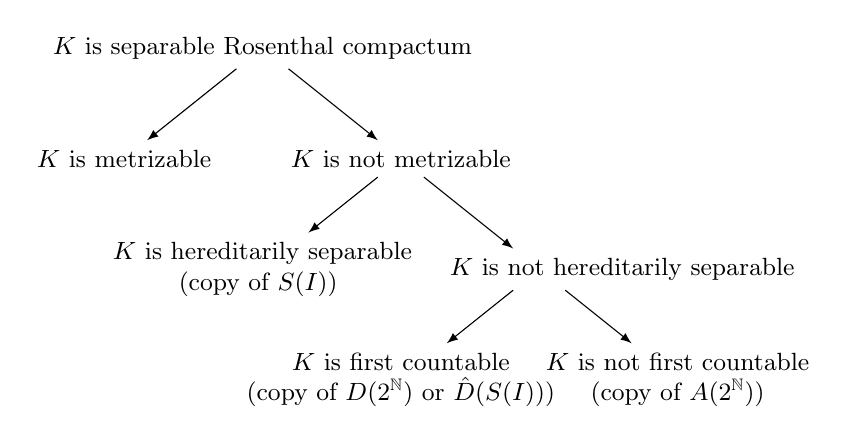
\begin{tikzpicture}[
  grow=down,
  sibling distance=10em,
  level distance=4em,
  edge from parent/.style={draw,-latex},
  every node/.style={font=\small,align=center}
  ]

\node {$K$ is separable Rosenthal compactum}
  child {node {$K$ is metrizable}
  }
  child {node {$K$ is not metrizable}
    child {node {$K$ is hereditarily separable \\ (copy of $S(I)$) \hspace{2cm}}}
    child {node {\hspace{2cm} $K$ is not hereditarily separable}
      child {node {$K$ is first countable \\ (copy of $D(2^\mathbb{N})$ or $\hat{D}(S(I))$)}}
      child {node {$K$ is not first countable \\ (copy of $A(2^\mathbb{N})$)}}
    }
  };

\end{tikzpicture}
\end{center}

The definitions provided here for NIP$_i$ ($i=1,2,3$) are topological. This raises the following question:

\begin{question}
    Is there a non-topological characterization for NIP$_i$, $i=1,2,3$?
\end{question}


\subsection{The Argyros-Dodos-Kanellopoulos heptachotomy, and approximability of deep computation by minimal classes}

%More can be said about the nature of the embeddings in Todorčević's Trichotomy. For an arbitrary separable Rosenthal compactum $K$, there is typically more than one countable dense subset of $K$. We can view a separable Rosenthal compactum as the accumulation points of a countable family of pointwise bounded real-valued functions. The choice of the countable families is not important when a bijection between them can be lifted to a homeomorphism of their closures. To be more precise:



In the three separable three cases given in \ref{E:Rosenthal comacta}, namely, ($\hat{A}(2^\mathbb{N})$, $S(2^\mathbb{N})$ and $\hat{D}(S(2^\mathbb{N}))$), the countable dense subsets are indexed by the binary tree $2^{<\mathbb{N}}$. This choice of index is useful for two reasons:
\begin{enumerate}
\item
Our emphasis is computational. Elements of $2^{<\mathbb{N}}$ represent finite bitstrings, i.e.,  standard computations, while Rosenthal compacta represent deep computations, i.e., limits of finite computations. Mathematically, deep computations are pointwise limits of standard computations. Howwever, computationally, we are interested in the manner (and the efficiency) in which the approximations can occur.
\item
The Ramsey theory of perfect subsets of the Cantor space $2^\mathbb{N}$ can be imported to analyze the behavior of the accumulation points. Since $2^{<\mathbb{N}}$ is countable, we can always choose this index for the countable dense subsets. This is done in \cite{argyros2008rosenthal}.
\end{enumerate}

\begin{defn}
Let $X$ be a Polish space.

\begin{enumerate}
\item
If  $I$ is a countable and $\{f_i:i\in I\}\subseteq\mathbb{R}^X$, $\{g_i:i\in I\}\subseteq\mathbb{R}^X$  are two pointwise families by  $I$, we say that $\{f_i:i\in\ I\}$ and $\{g_i:i\in I\}$ are \emph{equivalent} if and only if the map $f_i\mapsto g_i$ is extended to a homeomorphism from $\overline{\{f_i:i\in I\}}$ to $\overline{\{g_i:i\in I\}}$.
\item
If $\{f_t:t\in 2^{<\mathbb{N}}\}$ is a pointwise bounded family, we say that $\{f_t:t\in 2^{<\mathbb{N}}\}$ is \emph{minimal} if and only if for every dyadic subtree $\{s_t:t\in 2^{<\mathbb{N}}\}$ of $2^{<\mathbb{N}}$, $\{f_{s_t}:t\in 2^{<\mathbb{N}}\}$ is equivalent to $\{f_t:t\in 2^{<\mathbb{N}}\}$.
 \end{enumerate}
\end{defn}

One of the main results in \cite{argyros2008rosenthal} is that, up to equivalence,  there are  seven minimal families of Rosenthal compacta and that for every relatively compact $\{f_t:t\in 2^{<\mathbb{N}}\}\subseteq B_1(X)$ there is a dyadic subtree $\{s_t:t\in 2^{<\mathbb{N}}\}$ such that $\{f_{s_t}:t\in 2^{<\mathbb{N}}\}$ is equivalent to one of the minimal families. We shall describe the seven minimal families next. We follow the same notation as in \cite{argyros2008rosenthal}. For any node $t\in 2^{<\mathbb{N}}$, let us denote by $t^\frown 0^{\infty}$ ($t^\frown 1^{\infty}$) the infinite binary sequence starting with $t$ and continuing will all $0$'s (respectively, all $1$'s). Fix a regular dyadic subtree $R=\{s_t:t\in 2^{<\mathbb{N}}\}$ of $2^{<\mathbb{N}}$ (i.e., a dyadic subtree such that every level of $R$ is contained in a level of $2^{<\mathbb{N}}$) with the property that for all $s,s'\in R$, $s^\frown 0^{\infty}\neq s'^\frown 0^\infty$ and $s^\frown 1^{\infty}\neq s'^\frown 1^\infty$. Given $t\in 2^{<\mathbb{N}}$, let $v_t$ be the characteristic function of the set $\{x\in 2^\mathbb{N}:x \text{ extends } t\}$. Let $<$ be the lexicographic order in $2^\mathbb{N}$. Given $a\in 2^{\mathbb{N}}$, let $f^+_a:2^{\mathbb{N}}\rightarrow\{0,1\}$ be the characteristic function of $\{x\in 2^{\mathbb{N}}:a\leq x\}$ and let $f^-_a:2^{\mathbb{N}}\rightarrow\{0,1\}$ be the characteristic function of $\{x\in 2^{\mathbb{N}}:a<x\}$. Given two maps $f,g:2^{\mathbb{N}}\rightarrow\mathbb{R}$ we denote by $(f,g):2^{\mathbb{N}}\sqcup 2^{\mathbb{N}}\rightarrow\mathbb{R}$ the function which is $f$ on the first copy of $2^{\mathbb{N}}$ and $g$ on the second copy of $2^{\mathbb{N}}$.

\begin{enumerate}
    \item $D_1=\{\frac{1}{|t|+1}v_t:t\in 2^{<\mathbb{N}}\}$. This is discrete in $\overline{D_1}=A(2^{\mathbb{N}})$. 
    \item $D_2=\{s_t^\frown 0^{\infty}:t\in 2^{<\mathbb{N}}\}$. This is discrete in $\overline{D_2}=2^{\leq N}$.
    \item $D_3=\{f^+_{s_t^\frown 0^\infty}:t\in 2^{<\mathbb{N}}\}$. This is a discrete in $\overline{D_3}=S(2^{\mathbb{N}})$.
    \item $D_4=\{f^-_{s_t^\frown 1^\infty}:t\in 2^{<\mathbb{N}}\}$. This is discrete in $\overline{D_4}=S(2^{\mathbb{N}})$.
    \item $D_5=\{v_t:t\in 2^{<\mathbb{N}}\}$. This is discrete in $\overline{D_5}=\hat{A}(2^{\mathbb{N}})$.
    \item $D_6=\{(v_{s_t},s_t^\frown 0^\infty):t\in 2^{<\mathbb{N}}\}$. This is discrete in $\overline{D_6}=\hat{D}(2^{\mathbb{N}})$.
    \item $D_7=\{(v_{s_t},x^+_{s_t^\frown 0^\infty}):t\in 2^{<\mathbb{N}}\}$. This is discrete in $\overline{D_7}=\hat{D}(S(2^{\mathbb{N}}))$
\end{enumerate}

\begin{thm}[Heptacotomy of minimal families, Theorem 2 in \cite{argyros2008rosenthal}]
    Let $X$ be Polish. For every relatively compact $\{f_{t}:t\in 2^{<\mathbb{N}}\}\subseteq B_1(X)$, there exists $i=1,2,\dots, 7$ and a regular dyadic subtree $\{s_t:t\in 2^{<\mathbb{N}}\}$ of $2^{<\mathbb{N}}$ such that $\{f_{s_t}:t\in 2^{<\mathbb{N}}\}$ is equivalent to $D_i$. Moreover, all $D_i$ are minimal and mutually non-equivalent.
\end{thm}

\section{Measure-theoretic versions of NIP and universal Monte Carlo computability of  deep computations}
\label{Measure-theoretic NIP}

We now turn to the question: what happens when $\mathcal{P}$ is uncountable? Notice that the countability assumption is crucial in the proof of Theorem \ref{Generalized BFT} essentially because it makes $\mathbb{R}^\mathcal{P}$ a Polish space. For the uncountable case, we may lose Baire-1 definability so we shall replace $B_1(X)$ by a larger class. 

\subsection{A measure-theoretic version of NIP}

Recall that the \emph{raison d'être} of the class of Baire-1 functions is to have a class that is contains the continuous functions but is closed under pointwise limits, and that ( Fact~\ref{baire}) for perfectly normal $X$, a function  $f$ is in $B_1(X,Y)$ if and only if $f^{-1}[U]$ is an $F_\sigma$ subset of $X$ for every open $U\subseteq Y$. This motivates the following definition:



\begin{defn}
\label{D:universal measurability}
Given a Hausdorff space $X$ and a measurable space $(Y,\Sigma)$, we say that $f:X\rightarrow Y$ is \emph{universally measurable} (with respect to $\Sigma$) if $f^{-1}(E)$ is Borel for every $E\in\Sigma$, i.e., $f^{-1}(E)$ is $\mu$-measurable for every Radon measure $\mu$ on $X$. When $Y=\mathbb{R}$ we will always take $\Sigma=\mathcal{B}(\mathbb{R})$, the Borel $\sigma$-algebra of $\mathbb{R}$. 
\end{defn}

\begin{rem} 
A function $f:X\rightarrow\mathbb{R}$ is universally measurable if and only if $f^{-1}(U)$ is $\mu$-measurable for every Radon probability measure $\mu$ on $X$ and every open set $U\subseteq\mathbb{R}$. 
\end{rem}

Intuitively,  a function is universally measurable if it is ``measurable no matter which reasonable way you try to measure things on its domain". The concept of universal measurability emerged from work of  Kallianpur and Sazonov, in the late 1950's and 1960s, , with later developments by Blackwell, Darst, and others, building on earlier ideas of Gnedenko and Kolmogorov from the 1950s.  See~\cite[Chapters 1 and 2]{Pap:2002}.

%In \cite{BFT_1978_PCompactBaire}, J. Bourgain, D.H. Fremlin and M. Talagrand characterized the Non-Independence Property of a set of continuous functions with various notions of compactness in function spaces containing $C(X)$, such as $B_1(X)$. In this section we will replace $B_1(X)$ with the larger space $M_r(X)$ of universally measurable functions. The development of this section is based on Theorem 2F in \cite{BFT_1978_PCompactBaire}. We now give the relevant definitions. Readers with limited familiarity with measure theory may refer to the appendix for standard definitions appearing in this subsection.
%

\begin{notn}
Following \cite{BFT_1978_PCompactBaire}, the collection of all universally measurable real-valued functions will be denoted by $M_r(X)$. 
\end{notn}

In the context of deep computations, we will be interested in transition maps from a state space $L\subseteq \mathbb{R}^\mathcal{P}$ to itself. There are two natural $\sigma$-algebras one can consider in the product space $\mathbb{R}^\mathcal{P}$: the Borel $\sigma$-algebra, i.e., the $\sigma$-algebra generated by open sets in $\mathbb{R}^\mathcal{P}$, and the cylinder $\sigma$-algebra, i.e., the $\sigma$-algebra generated by the sub-basic open sets in $\mathbb{R}^\mathcal{P}$. Note that when $\mathcal{P}$ is countable, both $\sigma$-algebras coincide, but in general the cylinder $\sigma$-algebra is strictly smaller. We will use the cylinder $\sigma$-algebra to define universally measurable maps $f:\mathbb{R}^\mathcal{P}\rightarrow\mathbb{R}^\mathcal{P}$. The reason for this choice is the following characterization:

\begin{lem}\label{lemma:coordinated_univ_meas}
    Let $X$ be a Hausdorff space and $Y=\prod_{i\in I}Y_i$ be any product of measurable spaces $(Y_i,\Sigma_i)$ for $i\in I$. Let $\Sigma_Y$ be the cylinder $\sigma$-algebra generated by the measurable spaces $(Y_i,\Sigma_i)$. Let $f:X\rightarrow Y$. The following are equivalent:
    \begin{itemize}
        \item [(i)] $f:X\rightarrow Y$ is universally measurable (with respect to $\Sigma_Y$).
        \item [(ii)] $\pi_i\circ f:X\rightarrow Y_i$ is universally measurable (with respect to $\Sigma_i$) for all $i\in I$.
    \end{itemize}
\end{lem}

\begin{proof}
    (i)$\Rightarrow$(ii) is clear since the projection maps $\pi_i$ are measurable and the composition of measurable functions is measurable. To prove (ii)$\Rightarrow$(i), suppose that $C=\prod_{i\in I}C_i$ is a measurable cylinder and let $J$ be the finite set of $i\in I$ such that $C_i\neq Y_i$. Then, $C=\bigcap_{i\in J}\pi_i^{-1}(C_i)$, so $f^{-1}(C)=\bigcap_{i\in J}(\pi_i\circ f)^{-1}(C_i)$ is a universally measurable set by assumption.
\end{proof}

The preceding lemma says that a transition map is universally measurable if and only if it is universally measurable on all its features. In other words, we can check measurability of a transition just by checking measurability feature by feature. We will denote by $M_r(X,\mathbb{R}^\mathcal{P})$ the collection of all universally measurable functions $f:X\rightarrow\mathbb{R}^\mathcal{P}$ (with respect to the cylinder $\sigma$-algebra), endowed with the topology of pointwise convergence.

We will need the following result about NIP and universally measurable functions:

\begin{thm}[Bourgain-Fremlin-Talagrand, Theorem 2F in \cite{BFT_1978_PCompactBaire}]\label{BFT-2F}
    Let $X$ be a Hausdorff space and $A\subseteq C(X)$ be pointwise bounded. The following are equivalent:
    \begin{itemize}
        \item [(i)] $\overline{A}\subseteq M_r(X)$.
        \item [(ii)] For every compact $K\subseteq X$, $A|_K$ satisfies the NIP.
        \item [(iii)] For every Radon measure $\mu$ on $X$, $A$ is relatively countably compact in $\mathscr{M}^0(X,\mu)$, i.e., every countable subset of $A$ has an accumulation point in $\mathscr{M}^0(X,\mu)$. 
    \end{itemize}
\end{thm}


\subsection{Universal Monte Carlo computability of  deep computations}

We now wish to define the concept of a deep computation being computable except  a set of arbitrarily small measure ``no matter which reasonable way you try to measure things on its domain"  (see the remarks following definition~\label{D:universal measurability}). This is the concept of \emph{universal Monte Carlo computability} defined below (Definition~\label{D:universally essentially computable}). To motivate the definition, we need to recall two facts:

\begin{enumerate}
\item
Littlewoood's second principle states that every Lebesgue measurable function is ``nearly continuous''. The formal version of this, which is Luzin's theorem, states that if
 $(X,\Sigma ,\mu )$  a Radon measure space and $Y$ be a second-countable topological space (e.g., $Y=\mathbb{R}^\mathcal{P}$ with $\mathcal{P}$ countable ) equipped with a Borel algebra, then any given $f:X\to Y$ is measurable if and only if for every  $E\in\Sigma$ and every $\varepsilon>0$ there exists a closed $F\subseteq E$ such that the restriction $f|F$ is continuous.
\item
Computability of deep computations can is characterized in terms of continuous extendibility of computations. This is at the core of~\cite{alva2024approximability}.
\end{enumerate}


These facts motivate the following definition:


\begin{defn}
\label{D:universally essentially computable}
    Let $(L,\mathcal P,\Gamma)$ be a CCS. We say that a transition $f:L\rightarrow L$ is \emph{universally Monte Carlo computable} if and only if there exists $\tilde f:\mathcal{L}_{\text{sh}}\rightarrow \mathcal{L}_{\text{sh}}$ extending $f$ such that for every sizer $r_\bullet$ there is a sizer $s_\bullet$ such that the restriction $\tilde f|_{\mathcal{L}[r_{\bullet}]}:\mathcal{L}[r_\bullet]\rightarrow\mathcal{L}[s_\bullet]$ is universally measurable, i.e., $\pi_P\circ \tilde f|_{\mathcal{L}[r_{\bullet}]}:\mathcal{L}[r_\bullet]\rightarrow [-s_P,s_P]$ is $\mu$-measurable for every Radon probability measure $\mu$ on $\mathcal{L}[r_\bullet]$.
\end{defn}


\subsection{Bourgain-Fremlin-Talagrand, NIP, and universal Monte Carlo computability of  deep computations}



Theorem~\ref{BFT-2F} immediately yields the following.

\begin{thm}
    Let $(L,\mathcal P,\Gamma)$ be a CCS satisfying the Extendability Axiom. Let $R$ be an exhaustive collection of sizers. Let $\Delta\subseteq\Gamma$ be $R$-confined. If $\pi_P\circ\Delta|_{L[r_\bullet]}$ satisfies the NIP for all $P\in\mathcal{P}$ and all $r_{\bullet}\in R$, then every deep computation is universally Monte Carlo computable.
\end{thm}

\begin{proof}
    By the Extendability Axiom, Theorem \ref{BFT-2F} and lemma \ref{NIP and closure} we have that $\overline{\pi_P\circ\tilde\Delta|_{\mathcal{L}[r_\bullet]}}\subseteq M_r(\mathcal{L}[r_\bullet])$ for all $r_\bullet\in R$ and $P\in\mathcal{P}$. Let $f\in\overline{\Delta}$ be a deep computation. Write $f=\mathcal{U}\lim_i\gamma_i$ as an ultralimit of computations in $\Delta$. Define $\tilde f:=\mathcal{U}\lim_i\tilde\gamma_i$. Then, for all $r_\bullet\in R$ and $P\in\mathcal{P}$ $\pi_P \circ \tilde\gamma_i|_{\mathcal{L}[r_\bullet]}\in M_r(\mathcal{L}[r_\bullet])$ for all $i$, so $\pi_P \circ f|_{\mathcal{L}[r_\bullet]}\in \overline{\pi_P\circ\tilde\Delta|_{\mathcal{L}[r_\bullet]}}\subseteq M_r(\mathcal{L}[r_\bullet])$.
\end{proof}

\begin{question}
Under the same assumptions of the preceding theorem, suppose that every deep computation of $\Delta$ is universally Monte Carlo computable. Must $\pi_P\circ\Delta|_{L[r_\bullet]}$ have the NIP for all $P\in\mathcal{P}$ and all $r_{\bullet}\in R$?
\end{question}

\subsection{Talagrand stability, Fremiln's dichotomy, NIP, and universal Monte Carlo computability of  deep computations}

There is another notion closely related to NIP, introduced by Talagrand in \cite{talagrand1984pettis} while studying Pettis integration. Suppose that $X$ is a compact Hausdorff space and $A\subseteq \mathbb{R}^X$. Let $\mu$ be a Radon probability measure on $X$. Given a $\mu$-measurable set $E\subseteq X$, a positive integer $k$ and real numbers $a<b$. we write:

$$D_k(A,E,a,b)=\bigcup_{f\in A}\{x\in E^{2k}:f(x_{2i})\leq a, \hspace{1mm} f(x_{2i+1})\geq b \hspace{1mm}{\text{ for all }i<k} \}$$

We say that $A$ is \emph{Talagrand $\mu$-stable} if and only if for every $\mu$-measurable set $E\subseteq X$ of positive measure and for every $a<b$ there is $k\geq 1$ such that
\[
(\mu^{2k})^*(D_k(A,E,a,b))<(\mu(E))^{2k},
\]
where $\mu*$ denotes the outer measure (we work with outer since the sets $D_k(A,E,a,b)$ need not be $\mu$-measurable). This is certainly the case when $A$ is a countable set of continuous (or $\mu$-measurable) functions. 

\begin{notn}
For a measure $\mu$ on a set $X$, the set of all $\mu$-measurable functions will  denoted by $\mathscr{M}^0(X,\mu)$.
\end{notn}

The following lemma establishes that Talagrand stability is a way to ensure that deep computations are definable by measurable functions. We include a proof for the reader's convenience.

\begin{lem}\label{talagrand stable is relatively compact}
    If $A$ is Talagrand $\mu$-stable, then $\overline{A}$ is also Talagrand $\mu$-stable and $\overline{A}\subseteq\mathscr{M}^0(X,\mu)$.
\end{lem}

\begin{proof}
    First, observe that a subset of a $\mu$-stable set is $\mu$-stable. To show that $\overline{A}$ is $\mu$-stable, observe that $D_k(\overline{A},E,a,b)\subseteq D_k(A,E,a',b')$ where $a<a'<b'<b$ and $E$ is a $\mu$-measurable set with positive measure. It suffices to show that $\overline{A}\subseteq \mathscr{M}^0(X,\mu)$. Suppose that there exists $f\in\overline{A}$ such that $f\notin \mathscr{M}^0(X,\mu)$. By a characterization of measurable functions (see 413G in \cite{fremlin2003vol4}), there exists a $\mu$-measurable set $E$ of positive measure and $a<b$ such that $\mu^*(P)=\mu^*(Q)=\mu(E)$ where $P=\{x\in E: f(x)\leq a\}$ and $Q=\{x\in E: f(x)\geq b\}$. Then, for any $k\geq 1$: $(P\times Q)^k\subseteq D_k(\{f\},E,a,b)$ so $(\mu^{2k})^*(D_k(\{f\},E,a,b))=(\mu^*(P)\mu^*(Q))^k=(\mu(E))^{2k}$. Thus, $\{f\}$ is not $\mu$-stable, but we argued before that a subset of a $\mu$-stable set must be $\mu$-stable.
\end{proof}

We say that $A$ is \emph{universally Talagrand stable} if $A$ is Talagrand $\mu$-stable for every Radon probability measure $\mu$ on $X$. An argument similar to the proof of~\ref{BFT-2F}, yields the following:

\begin{thm}
    Let $(L,\mathcal P,\Gamma)$ be a CCS satisfying the Extendability Axiom. If $\pi_P\circ\Delta|_{L[r_\bullet]}$ is universally Talagrand stable for all $P\in\mathcal{P}$ and all sizers $r_{\bullet}$, then every deep computation is universally Monte Carlo computable.
\end{thm}

It is then natural to ask: what is the relationship between Talagrand stability and the NIP? The following dichotomy will be useful.

\begin{lem}[Fremlin's Dichotomy, 463K in \cite{fremlin2003vol4}]
\label{T:Fremlins dichotomy}
    If $(X,\Sigma,\mu)$ is a perfect $\sigma$-finite measure space (in particular, for $X$ compact and $\mu$ a Radon probability measure on $X$) and $\{f_n:n\in\mathbb{N}\}$ be a sequence of real-valued measurable functions on $X$, then either
    \begin{itemize}
        \item [(i)] $\{f_n:n\in\mathbb{N}\}$ has a subsequence that converges $\mu$-almost everywhere, or
        \item [(ii)] $\{f_n:n\in\mathbb{N}\}$ has a subsequence with no $\mu$-measurable accumulation point in $\mathbb{R}^X$.
    \end{itemize}
\end{lem}

The preceding lemma can be considered as a measure-theoretic version of Rosenthal's Dichotomy. Combining this dichotomy with Theorem \ref{BFT-2F}, we get the following result:

\begin{thm}
    Let $X$ be a Hausdorff space and $A\subseteq C(X)$ be pointwise bounded. The following are equivalent:
    \begin{itemize}
        \item [(i)] $\overline{A}\subseteq M_r(X)$.
        \item [(ii)] For every compact $K\subseteq X$, $A|_K$ satisfies the NIP.
        \item [(iii)] For every Radon measure $\mu$ on $X$, $A$ is relatively countably compact in $\mathscr{M}^0(X,\mu)$, i.e., every countable subset of $A$ has an accumulation point in $\mathscr{M}^0(X,\mu)$.
        \item [(iv)] For every Radon measure $\mu$ on $X$ and every sequence $\{f_n:n\in\mathbb{N}\}\subseteq A$, there is a subsequence that converges $\mu$-almost everywhere.
    \end{itemize}
\end{thm}

\begin{proof}
    Notice that the equivalence (i)-(iii) is Theorem \ref{BFT-2F}. Notice that the equivalence of (iii) and (iv) is Fremlin's Dichotomy (Theorem~\ref{T:Fremlins dichotomy}).
\end{proof}

Finally, it is natural to ask what the connection is between Talagrand stability and NIP.

\begin{prop}
    Let $X$ be a compact Hausdorff space and $A\subseteq C(X)$ be pointwise bounded. If $A$ is universally Talagrand stable, then $A$ satisfies the NIP.
\end{prop}

\begin{proof}
    By Theorem \ref{BFT-2F}, it suffices to show that $A$ is relatively countably compact in $\mathscr{M}^0(X,\mu)$ for all Radon probability measure $\mu$ on $X$. Since $A$ is Talagrand $\mu$-stable for any such $\mu$, we have $\overline{A}\subseteq\mathscr{M}^0(X,\mu)$. In particular, $A$ is relatively countably compact in $\mathscr{M}^0(X,\mu)$.
\end{proof}

\begin{question}
    Is the converse true?
\end{question}

The following two results suggest that the precise connection between Talagrand stability and NIP may be sensitive to set-theoretic axioms (even assuming countability of $A$).

\begin{thm}[Talagrand, Theorem 9-3-1(a) in \cite{talagrand1984pettis}]
    Let $X$ be a compact Hausdorff space and $A\subseteq M_r(X)$ be countable and pointwise bounded. Assume that $[0,1]$ is not the union of $<\mathfrak{c}$ closed measure zero sets. If $A$ satisfies the NIP, then $A$ is universally Talagrand stable.
\end{thm}

\begin{thm}[Fremlin, Shelah, \cite{fremlin1993pointwise}]
    It is consistent that there exists a countable pointwise bounded set of Lebesgue measurable functions with the NIP which is not Talagrand stable with respect to Lebesgue measure.
\end{thm}


\begin{comment}

\section*{Appendix: Measure Theory}

Given a set $X$, a collection $\Sigma$ of subsets of $X$ is called a \emph{$\sigma$-algebra} if $\Sigma$ contains $X$ and is closed under complements and countable unions. Hence, for example, a $\sigma$-algebra is also closed under countable intersections. Intuitively, a $\sigma$-algebra is a collection of sets in which we can define a $\sigma$-additive measure. We call sets in a $\sigma$-algebra $\Sigma$ \emph{measurable sets} and the pair $(X,\Sigma)$ a measurable space. If $X$ is a topological space, there is a natural $\sigma$-algebra of subsets of $X$, namely the \emph{Borel $\sigma$-algebra} $\mathcal{B}(X)$, i.e., the smallest $\sigma$-algebra containing all open subsets of $X$. Given two measurable spaces $(X,\Sigma_X)$ and $(Y,\Sigma_Y)$, we say that a function $f:X\rightarrow Y$ is \emph{measurable} if and only if $f^{-1}(E)\in\Sigma_X$ for every $E\in \Sigma_Y$. In particular, we say that $f:X\rightarrow\mathbb{R}$ is measurable if $f^{-1}(E)\in \Sigma_X$ for all $E\in\mathcal{B}(\mathbb{R})$ (equivalently, $E$ open in $\mathbb{R}$).

Given a measurable space $(X,\Sigma)$, a \emph{$\sigma$-additive measure} is a non-negative function $\mu:\Sigma\rightarrow\mathbb{R}$ with the property that $\mu(\emptyset)=0$ and $\mu(\bigcup_{n=0}^\infty A_n)=\sum_{n=0}^\infty\mu(A_n)$ whenever $\{A_n:n\in\mathbb{N}\}\subseteq\Sigma$ is pairwise disjoint. We call $(X,\Sigma,\mu)$ a \emph{measure space}. A $\sigma$-additive measure is called a \emph{probability measure} if $\mu(X)=1$. A measure $\mu$ is \emph{complete} if for every $A\subseteq B\in\Sigma$, $\mu(B)=0$ implies $A\in\Sigma$. In words, subsets of measure-zero sets are always measurable (and hence, by the monotonicity of $\mu$, have measure zero as well). A measure $\mu$ is \emph{$\sigma$-finite} if $X=\cup_{n=1}^\infty X_n$ where $\mu(X_n)<\infty$ for all $n\in\mathbb{N}$ (i.e., $X$ can be decomposed into countably many finite measure sets). A measure $\mu$ is \emph{perfect} if for every measurable $f:X\rightarrow\mathbb{R}$ and every measurable set $E$ with $\mu(E)>0$, there exists a compact $K\subseteq f(E)$ such that $\mu(f^{-1}(K))>0$. We say that a property $\phi(x)$ about $x\in X$ holds \emph{$\mu$-almost everywhere} if $\mu(\{x\in X:\varphi(x) \text{ does not hold}\})=0$.

A special example of the preceding concepts is that of a \emph{Radon measure}. If $X$ is a Hausdorff topological space, then a measure $\mu$ on the Borel sets of $X$ is called a \emph{Radon measure} if
\begin{itemize}
    \item for every open set $U$, $\mu(U)$ is the supremum of $\mu(K)$ over all compact $K\subseteq U$, that is, the measure of open sets may be approximated via compact sets; and
    \item every point of $X$ has a neighborhood $U\ni x$ for which $\mu(U)$ is finite.
\end{itemize}

The most famous nontrivial example of a Radon measure on $\mathbb R$ is the Lebesgue measure of Borel sets. If $X$ is finite, $\mu(A):=|A|$ (the cardinality of $A$) defines a Radon measure on $X$. Every Radon measure is perfect (see 451A, 451B and 451C in \cite{fremlin2003vol4}).

While not immediately obvious, sets can be measurable according to one measure, but non-measurable according to another. Given a measure space $(X,\Sigma,\mu)$ we say that a set $E\subseteq X$ is \emph{$\mu$-measurable} if there are $A,B\in \Sigma$ such that $A\subseteq E\subseteq B$ and $\mu(B\backslash A)=0$. The set of all $\mu$-measurable sets is a $\sigma$-algebra containing $\Sigma$ and it is denoted by $\Sigma_\mu$. A set $E\subseteq X$ is \emph{universally measurable} if it is $\mu$-measurable for every Radon probability measure on $X$. It follows that Borel sets are universally measurable. We say that $f:X\rightarrow\mathbb{R}$ is \textit{$\mu$-measurable} if $f^{-1}(E)\in\Sigma_\mu$ for all $E\in\mathcal{B}(\mathbb{R})$ (equivalently, $E$ open in $\mathbb{R}$). 

Recall that if $\{X_i:i\in I\}$ is a collection of topological spaces indexed by some set $I$, then the product space $X:=\prod_{i\in I}X_i$ is endowed with the topology generated by \emph{cylinders}, that is, sets of the form $\prod_{i\in I} U_i$ where each $U_i$ is open in $X_i$, and $U_i=X_i$ except for finitely many indices $i\in I$. If each space is measurable, say we pair $X_i$ with a $\sigma$-algebra $\Sigma_i$, then there are multiple ways to interpret the product space $X$ as a measurable space, but the interpretation we care about in this paper is the so called \emph{cylinder $\sigma$-algebra}, as used in Lemma~\ref{lemma:coordinated_univ_meas}. Namely, let $\Sigma$ be the $\sigma$-algebra generated by sets of the form $$\prod_{i\in I}C_i,\quad C_i\in\Sigma_i,\ C_i=X_i\ \text{for all but finitely many }i\in I.$$

We remark that when $I$ is uncountable and $\Sigma_i=\mathcal B(X_i)$ for all $i\in I$, then $\Sigma$ is, in general, strictly \textbf{smaller} than $\mathcal B(X)$.


\end{comment}

%%%%%%%%%%%%%%%%%%%%%%%%%%%%%%%%%%%%%%%%%%%%%%%%%%%%%%%%%%%%%%%%%%%%%%%%%%

%Proof below was simplified by the previous

%\begin{thm}
    %Let $X$ be a Polish space, $\mathcal{P}$ be a countable set and $Y=\mathbb R^\mathcal P$. Let $A\subseteq C_p(X,Y)$ be a pointwise bounded set (i.e. for all $x\in X$, there is a sizer $r_{\bullet}^x=\{r_P^x\}_{P\in\mathcal{P}}$ such that for all $f\in A$ and $P\in\mathcal P$, $\pi_P\circ f(x)\in[-r_P^x,r_P^x]$). The following are equivalent:

    %\begin{itemize}
        %\item [(i)] For every compact $K\subseteq X$, $A|_K$ is relatively compact in $B_1(K,Y)$.
        %\item [(ii)] For every compact $K\subseteq X$, $\overline{A|_K}\subseteq B_1(X,Y)$.
        %\item [(iii)] For every compact $K\subseteq X$, for every $P\in\mathcal P$, $\{f_n\}_n\subseteq A$ and reals $\alpha<\beta$, there is $I\subseteq\mathbb N$ such that for any $p\in\mathcal P'$,
    %$$
    %\bigcap_{n\in I}(p\circ f)^{-1}(-\infty,\alpha]\cap\bigcap_{n\notin I}(p\circ f)^{-1}[\beta,\infty)\cap K=\emptyset.
    %$$
        %\item [(iv)] For any relatively compact $L$, for any finite $\mathcal P'\subseteq\mathcal P$, $\{f_n\}_n\subseteq A$ and reals $\alpha<\beta$, there are disjoint finite sets $F,G\subseteq\mathbb N$ such that for any $p\in\mathcal P'$,$$\bigcap_{n\in F}(p\circ f)^{-1}(-\infty,\alpha]\cap\bigcap_{n\in G}(p\circ f)^{-1}[\beta,\infty)\cap L=\emptyset.$$
    %\end{itemize}
%\end{thm}



%\subsection{Proof of the conjecture}

%$\boxed{1\implies 2}$

%Denote $F:=A|_K$ and suppose that $f\in\overline F\setminus B_1(X,Y)$. Lemma 1 implies that $\hat f\notin B_1(\mathcal P\times X)$. Since $\mathcal P\times X$ is a Polish space, we apply Fact~\ref{baire} to find reals $\alpha<\beta$ and countable sets $D_0,D_1\subseteq\mathcal P\times X$ with $\overline{D_0}=\overline{D_1}$, $D_0\subseteq\hat f^{-1}(-\infty,\alpha]$ and $D_1\subseteq\hat f^{-1}[\beta,\infty)$.

%For each $p\in\mathcal P$ and $i<2$, let $D_i^p:=\{x\in X:(p,x)\in D_i\}$ and consider $D=\bigcup_{p\in\mathcal P}(D_0^p\cup D_1^p)$. Since $D$ is countable, enumerate it in order type $\omega$, $D=\{x_i:i<\omega\}$.

%This is Stevo's diagonal argument. For each $n\geq1$, find $f_n\in F$ such that the distance between $f(x_i)$ and $f_n(x_i)$ is less than $1/n$ for all $i\leq n$. Then, for all fixed $i<\omega$, if $n\geq i$, then for every fixed $x\in D$, $\lim_{n\to\infty}f_n(x)=f(x)$.

%$F$ is not just relatively compact, but relatively countably compact. Thus, let $g\in B_1(X,Y)$ be an accumulation point of $\{f_n\}_n$. It is clear that $f_D=g|_D$, since $g=\lim_{k\to\infty}f_{n_k}$, and thus for all $x\in D$, $g(x)=\lim_{k\to\infty}f_{n_k}(x)=\lim_{n\to\infty}f_n(x)=f(x)$.

%It follows that $D_0\subseteq\hat g^{-1}(-\infty,\alpha]$ and $D_1\subseteq\hat g^{-1}[\beta,\infty)$. Let $E:=\overline{D_0}=\overline{D_1}$. By Fact~\ref{baire}, $\hat g|_E$ must have a point of continuity $x\in E$. Let $\varepsilon:=\frac{\beta-\alpha}2>0$ and find $\delta>0$ such that $d(x,y)<\delta$ implies $|\hat g(x)-\hat g(y)|<\varepsilon$. By density arguments, find for each $i$ an $x_i\in D_i$, with $d(x,x_i)<\delta$. But then, the triangle inequality and the choice of $\alpha,\beta$ give $\beta-\alpha\leq|\hat g(x_0)-\hat g(x_1)|<\beta-\alpha$, a contradiction.

%$\boxed{2\implies 3}$

%To prove the remaining implication we need:

%\begin{lem}
    %$\overline{\hat A|_K}\setminus B_1(\mathcal P\times X)\neq\emptyset$ implies that $\overline{A|_K}\setminus B_1(X,Y)\neq\emptyset$.
%\end{lem}

%%%%%%%%%%%%%%%%%%%%%%%%%%%%%%%%%%%%%%%%%%%%%%%%%%%%%%%%%%%%%%%%%

%\begin{thebibliography}{9}



\bibliographystyle{alpha}
\nocite{*}
\bibliography{bib}

%\end{thebibliography}
\end{document}